\documentclass[a4paper,12pt]{report}
\usepackage{a4wide}

%\documentclass[a5paper,10pt]{book}
%\usepackage[top=23mm, bottom=18mm, left=15mm, right=25mm]{geometry}
%\geometry{papersize={170mm,220mm}}


\usepackage[utf8x]{inputenc}
\usepackage[danish]{babel}

\usepackage{xr-hyper} %Externe hyper-ref
\usepackage[colorlinks=true, hyperindex=true, linkcolor=minmblaa, citecolor=minmblaa, urlcolor=minmblaa]{hyperref}
\hypersetup{colorlinks=true,filecolor=minmblaa,bookmarksnumbered=true} %Til hyperreferencer. Referencer med farver
\usepackage{needspace} % giver mulighed for at kræve at der skal være et antal tomme linier på siden før ellers indsættes et sideskift.
\usepackage{framed} %Bokse
\usepackage{wrapfig}

\usepackage{amsmath,amsfonts,amssymb,amsthm,mathtools} %Matematikpakker

\setlength{\parindent}{0mm} %Ingen Indhak i første linje i afsnit

\usepackage{color} %Farvepakke

\usepackage{array}
\usepackage{colortbl}
\usepackage{multirow} %Til at flette rækker i tabeller.

\usepackage{verbatim,mhchem}



	% DOWNLOAD FRA: http://sarovar.org/frs/?group_id=52&release_id=97
	% Læg i directory for hoved TEX fil
%\usepackage[draft]{pdfdraftcopy}
%\draftstring{Licens: Kasper Langt Mellemnavn Skårhøj}
%\draftfontsize{30}
	%\draftfontfamily{hlh}
	%\draftangle{45}
	%\definecolor{mycolor}{rgb}{.825,.855,1}
	%\draftcolor{mycolor}
	%\draftfontattrib



% = Sidehoved =
\usepackage{fancyhdr}
\pagestyle{fancy}
\renewcommand{\sectionmark}[1]{\markright{\protect\titlegraphic{dturoed}\textcolor{dtugraa}{\thesection~\MakeUppercase{#1}}}} % \thesection.\
\fancyhead{}
\fancyfoot{}
\fancyhead[R]{\titlefont\thepage}
\fancyhead[C]{}
\fancyhead[L]{\titlefont \small eNote \MakeUppercase{~\thechapter}~\hspace*{1ex}\rightmark}
\renewcommand\headrulewidth{0pt}
\fancypagestyle{plain}{\fancyfoot[C]{}}% {\titlefont\footnotesize\thepage}}
\setlength{\headheight}{15pt}


% = Længder
%\newlength{\envtblsep}\setlength{\envtblsep}{1\FrameSep}
\newlength{\obsl}\setlength{\obsl}{\textwidth-1.2cm-13.2pt}

% Includes:

% =     Fonts (select one)    =
\usepackage{mathpazo}\linespread{1.05} % Palatino needs more leading (space between lines)
\usepackage{bm} % bold math, must be loaded after the fontpackages

% % Til overskrifter
\DeclareTextFontCommand{\th}{\fontencoding{T1}\fontfamily{phv}\fontseries{b}\selectfont}
\newcommand\titlefont{\fontencoding{T1}\fontfamily{phv}\selectfont}


% =     PGF grafik      =
\usepackage{tikz}
\newcommand\titlegraphic[1]{%
\tikz[baseline] %
\draw[thick,color=#1]
(0pt  ,-0.25em) -- (0pt  ,0.85em)
(2.5pt,-0.25em) -- (2.5pt,0.85em)
(5pt  ,-0.25em) -- (5pt  ,0.85em)
(7.5pt,-0.25em) -- (7.5pt,0.85em);\hspace*{0.8ex} %
}

\newcommand\titlegraphicwide[1]{%
\tikz[baseline] %
\draw[line width=0.8mm,color=#1]
(0pt  ,-0.25em) -- (0pt  ,0.85em)
(4.5pt,-0.25em) -- (4.5pt,0.85em)
(9pt  ,-0.25em) -- (9pt  ,0.85em)
(13.5pt,-0.25em) -- (13.5pt,0.85em);\hspace*{0.8ex} %
}


% =      Title Layout      =
\usepackage{titlesec}
\makeatletter
\titleformat{\chapter}
	[display] % Shape
	{\titlefont\Huge\flushleft} % Title and label format
	{\titlefont\LARGE\bfseries \titlegraphicwide{dturoed}\textcolor{dtugraa}{\@chapapp~\thechapter}} % label
	{0.9em} % label/title separation
	{} % before code
	[] % after code
\makeatother
\titleformat{\section}
	[hang] % Shape
	{\titlefont\Large\flushleft} % Title and label format
	{\thesection} % label
	{0.9em} % label/title separation
	{} % before code
	[] % after code
\titleformat{\subsection}
	[hang] % Shape
	{\titlefont\large} % Title and label format
	{\thesubsection} % label
	{0.9em} % label/title separation
	{} % before code
	[] % after code
\titlespacing{\subsection}{0pt}{*6}{*1.5}
\titleformat{\subsubsection}
	[hang] % Shape
	{\titlefont} % Title and label format
	{\thesubsubsection} % label
	{0.9em} % label/title separation
	{} % before code
	[] % after code



% = Farver
\definecolor{dturoed}{rgb}{0.6, 0.0, 0.0}
\definecolor{dtugraa}{rgb}{0.5, 0.5, 0.5}	% Lidt mørkere. Korrekt = 0.4
\definecolor{mingroenstreg}{rgb}{0.4,0.8,0}	% Sekundærfarve 14 : 102/204/0	(Forårsgrøn) -> Eksempler
\definecolor{mingroen}{rgb}{0.32,0.64,0}		% Sekundærfarve 14, 80% mørkere (tekst)
\definecolor{minorangestreg}{rgb}{1,0.6,0}		% Sekundærfarve 1 : 255/153/0	(Orange) -> Opgaver
\definecolor{minorange}{rgb}{0.8,0.48,0}		% Sekundærfarve 1 , 80% mørkere (tekst)

\definecolor{minblaa}{rgb}{0.2,0.4,0.8}	% Sekundærfarve 13 , 51/102/204 	( Blå -> Definitioner etc)
\definecolor{minmblaa}{rgb}{0.16,0.32,0.64}	% Sekundærfarve 13 , 80% mørkere (tekst)
\definecolor{thmbackground}{rgb}{0.97,.97, 0.99}	% Farve 13 - lys baggrund

\definecolor{mingraastreg}{rgb}{.5,.5,.5}
\definecolor{hvadbackground}{rgb}{0.97,.97, 0.97}
\definecolor{sumgul}{rgb}{1,1,.8}

\definecolor{hjmopgfarve}{rgb}{.96,1,.96}


% = Counter
\newcounter{evncount}[chapter]
\setcounter{evncount}{0}
\renewcommand{\theevncount}{\thechapter.\arabic{evncount}}
\renewcommand{\theequation}{\thechapter-\arabic{equation}}


% = Eksempler = example =
\newenvironment{example}[1][]{
	\refstepcounter{evncount}
	\setlength{\obsl}{\textwidth-1.2cm-13.2pt-9pt} % fix width of the info envirnment%
	\def\FrameCommand{ 
		\textcolor{mingroenstreg}{\vrule width 4pt} 
		\hspace{5pt} 
	}%
	\MakeFramed{\advance\hsize-\width \FrameRestore}%
	\needspace{3\baselineskip}
	\titlegraphic{mingroen}
	\textcolor{mingroen}{
		\th{Eksempel \theevncount \hspace*{5mm} #1}
	} 
	\vspace*{3mm}%
	\begin{small}
	\par
}
{
	\end{small}
	\endMakeFramed
}


% = Opgaver = exercise =
\newenvironment{exercise}[1][]{
	\refstepcounter{evncount}
	\setlength{\obsl}{\textwidth-1.2cm-13.2pt-9pt}% fix width of the info envirnment%
	\def\FrameCommand{
		\textcolor{minorangestreg}{\vrule width 4pt}
		\hspace{5pt}
	}%
	\MakeFramed{\advance\hsize-\width \FrameRestore}%
	\needspace{3\baselineskip}
	\titlegraphic{minorange}
	\textcolor{minorange}{
		\th{Opgave \theevncount \hspace*{5mm} #1}
	} 
	\vspace*{3mm}%
	\begin{small}
	\par
}
{
	\end{small}
	\endMakeFramed
}


% = Bevis
\newenvironment{bevis}{
	\setlength{\obsl}{\textwidth-1.2cm-13.2pt-9pt} % fix width of the info envirnment%
	\def\FrameCommand{
		\textcolor{mingraastreg}{\vrule width 4pt} 
		\hspace{5pt}
	}%
	\MakeFramed{\advance\hsize-\width \FrameRestore}%
	\needspace{3\baselineskip}
	\titlegraphic{black}
	\textcolor{black}{
		\th{Bevis}
	}
	\vspace*{3mm}%
	\begin{small}
	\par
}
{
	\bevisslut 
	\end{small}
	\endMakeFramed
}


% = Definition =
\newenvironment{definition}[1][]{
	\vspace{4mm}
	\pagebreak[1]
	\setlength{\obsl}{\textwidth-1.2cm-2\FrameSep-13.2pt}%
	\def\FrameCommand{
		\fboxsep=\FrameSep\fcolorbox{minblaa}{thmbackground}
	}
	\begin{minipage}{\textwidth}
	\MakeFramed{\advance\hsize-\width\FrameRestore}
	\refstepcounter{evncount}
	\titlegraphic{minblaa}
	\textcolor{minmblaa}{
		\th{Definition \theevncount \hspace*{5mm} #1}
	}
	\vspace*{3mm}
	\par
}
{
	\endMakeFramed 
	\end{minipage}
	\vspace{4mm}
}


% = Theorem =
\newenvironment{theorem}[1][]{
	\vspace{4mm}
	\pagebreak[1]%
	\setlength{\obsl}{\textwidth-1.2cm-2\FrameSep-13.2pt}%
	\def\FrameCommand{
		\fboxsep=\FrameSep\fcolorbox{minblaa}{thmbackground}
	}%
	\begin{minipage}{\textwidth}
	\MakeFramed{\advance\hsize-\width\FrameRestore}%
	\refstepcounter{evncount}
	\titlegraphic{minblaa}
	\textcolor{minmblaa}{
		\th{Sætning \theevncount \hspace*{5mm} #1}
	}
	\vspace*{3mm}
	\par
}
{
	\endMakeFramed 
	\end{minipage}
	\vspace{4mm}
}


% = Lemma =
\newenvironment{lemma}[1][]{
	\vspace{4mm}
	\pagebreak[1]
	\setlength{\obsl}{\textwidth-1.2cm-2\FrameSep-13.2pt}%
	\def\FrameCommand{
		\fboxsep=\FrameSep \fcolorbox{minblaa}{thmbackground}
	}
	\begin{minipage}{\textwidth} 
	\MakeFramed{\advance\hsize-\width \FrameRestore}
	\refstepcounter{evncount}
	\titlegraphic{minblaa}
	\textcolor{minmblaa}{
		\th{Hjælpesætning \theevncount \hspace*{5mm} #1}
	}
	\vspace*{3mm}
	\par
}
{
	\endMakeFramed 
	\end{minipage}
	\vspace{4mm}
}


% = Corollary =
\newenvironment{corollary}[1][]{
	\vspace{4mm}
	\pagebreak[1]
	\setlength{\obsl}{\textwidth-1.2cm-2\FrameSep-13.2pt}%
	\def\FrameCommand{
		\fboxsep=\FrameSep \fcolorbox{minblaa}{thmbackground}
	}
	\begin{minipage}{\textwidth} 
	\MakeFramed{\advance\hsize-\width \FrameRestore}
	\refstepcounter{evncount}
	\titlegraphic{minblaa}
	\textcolor{minmblaa}{
		\th{Følgesætning \theevncount \hspace*{5mm} #1}
	}
	\vspace*{3mm}
	\par
}
{
	\endMakeFramed 
	\end{minipage}
	\vspace{4mm}
}


% = Metode = method
\newenvironment{method}[1][]{
	\vspace{4mm}
	\pagebreak[1]
	\setlength{\obsl}{\textwidth-1.2cm-2\FrameSep-13.2pt}%
	\def\FrameCommand{
		\fboxsep=\FrameSep \fcolorbox{black}{hvadbackground}
	}
	\begin{minipage}{\textwidth} 
	\MakeFramed{\advance\hsize-\width \FrameRestore}
	\refstepcounter{evncount}
	\titlegraphic{black}
	\textcolor{black}{
		\th{Metode \theevncount \hspace*{5mm} #1}
	}
	\vspace*{3mm}
	\par
}
{
	\endMakeFramed
	\end{minipage}
	\vspace{4mm}
}


% = Forklaring = explain =
\newenvironment{explain}[1][]{
	\vspace{4mm}
	\pagebreak[1]
	\setlength{\obsl}{\textwidth-1.2cm-2\FrameSep-13.2pt}%
	\def\FrameCommand{
		\fboxsep=\FrameSep \fcolorbox{black}{hvadbackground}
	}
	\MakeFramed{\advance\hsize-\width \FrameRestore}
	\refstepcounter{evncount}
	\titlegraphic{black}
	\textcolor{black}{
		\th{Forklaring \theevncount \hspace*{5mm} #1}
	}
	\vspace*{3mm}
	\par
}
{
	\endMakeFramed
	\vspace{4mm}
}


% = Bemærkning = remark =
\newenvironment{remark}[1][]{
	\vspace{4mm}
	\pagebreak[1]
	\setlength{\obsl}{\textwidth-1.2cm-2\FrameSep-13.2pt}%
	\def\FrameCommand{
		\fboxsep=\FrameSep \fcolorbox{black}{hvadbackground}
	}
	\begin{minipage}{\textwidth} 
	\MakeFramed{\advance\hsize-\width \FrameRestore}
	\refstepcounter{evncount}
	\titlegraphic{black}
	\textcolor{black}{
		\th{Bemærkning \theevncount \hspace*{5mm} #1}
	}
	\vspace*{3mm}
	\par
}
{
	\endMakeFramed 
	\end{minipage}
	\vspace{4mm}
}







% = OBS! = obs =
\newenvironment{obs}{\vspace{4mm}\par%
\begin{tabular}{m{1.2cm}<{\hspace*{2mm}}@{}|m{\obsl}@{}}\hspace*{-4pt}\raggedleft
\includegraphics[width=1.1cm]{../Strukturfiler/FIGS/Alert01} & \begin{minipage}{\obsl}}{\end{minipage}\\ \end{tabular}\vspace{4mm}\par}


% = INFO = info =
\newenvironment{info}{\vspace{4mm}\par%
\begin{tabular}{m{1.2cm}<{\hspace*{2mm}}@{}|m{\obsl}@{}}\hspace*{-4pt}\raggedleft
\includegraphics[width=1.1cm]{../Strukturfiler/FIGS/Info01} & \begin{minipage}{\obsl}}{\end{minipage}\\ \end{tabular}\vspace{4mm}\par}


% = THINK= think =
\newenvironment{think}{\vspace{4mm}\par%
\begin{tabular}{m{1.2cm}<{\hspace*{2mm}}@{}|m{\obsl}@{}}\hspace*{-4pt}\raggedleft
\includegraphics[width=0.7cm]{../Strukturfiler/FIGS/ChessPiece} & \begin{minipage}{\obsl}}{\end{minipage}\\ \end{tabular}\vspace{4mm}\par}


% = AHA= aha =
\newenvironment{aha}{\vspace{4mm}\par%
\begin{tabular}{m{1.2cm}<{\hspace*{2mm}}@{}|m{\obsl}@{}}\hspace*{-4pt}\raggedleft
\includegraphics[width=1.1cm]{../Strukturfiler/FIGS/Think} & \begin{minipage}{\obsl}}{\end{minipage}\\ \end{tabular}\vspace{4mm}\par}


% = BUILDUP= build =
\newenvironment{build}{\vspace{4mm}\par%
\begin{tabular}{m{1.2cm}<{\hspace*{2mm}}@{}|m{\obsl}@{}}\hspace*{-4pt}\raggedleft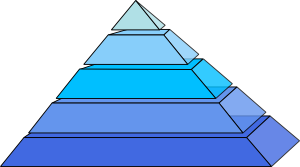
\includegraphics[width=1.1cm]{../Strukturfiler/FIGS/BluePyramid} & \begin{minipage}{\obsl}}{\end{minipage}\\ \end{tabular}\vspace{4mm}\newline}


% = Forudsætning = basis
\newenvironment{basis}{\begin{flushleft} \begin{itshape} }{\end{itshape} \end{flushleft}}


% = Opsummering =
\newenvironment{summary}{\clearpage\pagecolor{sumgul}\section{Opsummering}}{\newpage\pagecolor{white}}











% = Counter
\newcounter{opgavecount}[section]
\setcounter{opgavecount}{0}
\newcounter{spgcount}[opgavecount]
\setcounter{spgcount}{0}
\renewcommand{\thespgcount}{\alph{spgcount})}



% = EXERCISE = (DIVIDER)

\newcommand{\exercisebegin}[1][]{\bigskip\needspace{3\baselineskip}\refstepcounter{opgavecount}\titlegraphic{mingroen}\textcolor{mingroen}{\th{Opgave \theopgavecount \hspace*{1cm} #1}}\medskip\par}

% = QUIZEXERCISE = (DIVIDER)

\newcommand{\quizexercisebegin}[1][]{\bigskip\needspace{3\baselineskip}\refstepcounter{opgavecount}\titlegraphic{mingroen}\textcolor{mingroen}{\th{Quiz-Opgave \theopgavecount \hspace*{1cm} #1}}\medskip\par}

% = QUESTION =

\newenvironment{question}{\refstepcounter{spgcount}\begin{itemize}\item[\thespgcount]}{\end{itemize}\hspace*{\fill}}

% = VINK =

\newenvironment{vink}{\begin{tabular}{m{.9cm}<{\hspace*{2mm}}@{}|m{\obsl}@{}}\hspace*{-4pt}\raggedleft
\includegraphics[width=.9cm]{../Strukturfiler/FIGS/Think} & \begin{minipage}{\obsl}}{\end{minipage}\\ \end{tabular}\medskip\\}
	
% = FACIT =

\newenvironment{facit}{\begin{tabular}{m{.9cm}<{\hspace*{2mm}}@{}|m{\obsl}@{}}\hspace*{-4pt}\raggedleft
\includegraphics[width=.9cm]{../Strukturfiler/FIGS/Check} & \begin{minipage}{\obsl}}{\end{minipage}\\ \end{tabular}\medskip\\}








\newcommand{\afsnit}[1]{\bigskip\th{\titlegraphic{mingroen}\textcolor{mingroen}{#1}} \\ \rule[7pt]{.4\textwidth}{1pt} \vspace*{-2.5mm}\par}

% (DIVIDER):
\newcommand{\ugedagdatotitel}[4]{\pagebreak[4]\section{Semesteruge #1 -- #2 Dag \hspace*{1mm} (#3)} \vspace*{-4mm} \rule[5pt]{\textwidth}{1pt}\vspace*{-2.5mm} \begin{center}\large{\th{#4}}\end{center} \fancyhead[C]{\th{Semesteruge #1}}}

\newenvironment{skema}[1]{\definecolor{shadecolor}{rgb}{0.96,.98, 1.0} \setlength{\FrameSep}{6pt} \renewcommand{\FrameHeightAdjust}{10pt} \vspace*{-4pt}\begin{shaded} \begin{tabular}{#1}}{\end{tabular} \end{shaded} \vspace*{-7pt}}


% ========================

% MAKROER

%\newenvironment{matr}[1][]{\hspace*{-.8mm}\left[\hspace*{-1mm}\begin{array}{#1}}{\end{array}\hspace*{-1mm}\right]\hspace*{-.8mm}}
\newcommand{\bevisslut}{\begin{scriptsize} \begin{flushright} $ \blacksquare $ \end{flushright} \end{scriptsize}}

\newcommand{\tref}[2]{\hyperref[#1]{#2 \ref*{#1}}}
\newcommand{\thref}[2]{\hyperref[#1]{#2}}

\newcommand{\refA}[1]{\colorbox{yellow}{\ref{#1}}}
\newcommand{\hrefA}[2]{\colorbox{yellow}{\href{#1}{#2}}}
\newcommand{\trefA}[2]{\colorbox{yellow}{\hyperref[#1]{#2 \ref*{#1}}}}
\newcommand{\threfA}[2]{\colorbox{yellow}{\hyperref[#1]{#2}}}

\newenvironment{matr}[1]{\hspace*{-.8mm}\begin{bmatrix}\hspace*{-1mm}\begin{array}{#1}}{\end{array}\hspace*{-1mm}\end{bmatrix}\hspace*{-.8mm}}
\newcommand{\transp}{\hspace*{-.6mm}^{\top}}

\newcommand{\maengde}[2]{\left\lbrace \hspace*{-1mm} \begin{array}{c|c} #1 & #2 \end{array} \hspace*{-1mm} \right\rbrace}

\newenvironment{eqnalign}[1]{\setlength{\arraycolsep}{1.3pt}\begin{equation}\begin{array}{#1}}{\end{array}\end{equation}\par}
\newcommand{\eqnl}{\setlength{\arraycolsep}{1.3pt}}

\newcommand{\matind}[3]{{_\mathrm{#1}\mathbf{#2}_\mathrm{#3}}}
\newcommand{\vekind}[2]{{_\mathrm{#1}\mathbf{#2}}}
\newcommand{\jac}[2]{{\mathrm{Jacobi}_\mathbf{#1} (#2)}}
\newcommand{\diver}[2]{{\mathrm{div}\mathbf{#1} (#2)}}
\newcommand{\rot}[1]{{\mathbf{rot}\mathbf{(#1)}}}

\newcommand{\am}{\mathrm{am}}
\newcommand{\gm}{\mathrm{gm}}
\newcommand{\E}{\mathrm{E}}
\newcommand{\Span}{\mathrm{span}}
\newcommand{\mU}{\mathbf{U}}

\newcommand{\ms}{\medskip\\}
\newcommand{\bs}{\bigskip\\}

\newcommand{\mA}{\mathbf{A}}
\newcommand{\mB}{\mathbf{B}}
\newcommand{\mC}{\mathbf{C}}
\newcommand{\mD}{\mathbf{D}}
\newcommand{\mE}{\mathbf{E}}
\newcommand{\mF}{\mathbf{F}}
\newcommand{\mK}{\mathbf{K}}
\newcommand{\mI}{\mathbf{I}}
\newcommand{\mM}{\mathbf{M}}
\newcommand{\mN}{\mathbf{N}}
\newcommand{\mQ}{\mathbf{Q}}
\newcommand{\mT}{\mathbf{T}}
\newcommand{\mV}{\mathbf{V}}
\newcommand{\mW}{\mathbf{W}}
\newcommand{\mX}{\mathbf{X}}
\newcommand{\ma}{\mathbf{a}}
\newcommand{\mb}{\mathbf{b}}
\newcommand{\mc}{\mathbf{c}}
\newcommand{\md}{\mathbf{d}}
\newcommand{\me}{\mathbf{e}}
\newcommand{\mn}{\mathbf{n}}
\newcommand{\mr}{\mathbf{r}}
\newcommand{\mv}{\mathbf{v}}
\newcommand{\mw}{\mathbf{w}}
\newcommand{\mx}{\mathbf{x}}
\newcommand{\mxb}{\mathbf{x_{bet}}}
\newcommand{\my}{\mathbf{y}}
\newcommand{\mz}{\mathbf{z}}
\newcommand{\reel}{\mathbb{R}}
\newcommand{\mL}{\bm{\Lambda}} %Lambda-matrix
\newcommand{\mnul}{\bm{0}}
\newcommand{\trap}[1]{\mathrm{trap}(#1)}
\newcommand{\Det}{\operatorname{Det}}
\newcommand{\adj}{\operatorname{adj}}
\newcommand{\Ar}{\operatorname{Areal}}
\newcommand{\Vol}{\operatorname{Vol}}
\newcommand{\Rum}{\operatorname{Rum}}
\newcommand{\diag}{\operatorname{\bf{diag}}}
\newcommand{\bidiag}{\operatorname{\bf{bidiag}}}
\newcommand{\spanVec}[1]{\mathrm{span}\{#1\}}
\newcommand{\Div}{\operatorname{Div}}
\newcommand{\Rot}{\operatorname{\mathbf{Rot}}}

\newcommand{\Jac}{\operatorname{Jacobi}}
\newcommand{\Tan}{\operatorname{Tan}}
\newcommand{\Ort}{\operatorname{Ort}}
\newcommand{\Flux}{\operatorname{Flux}}
\newcommand{\Cmass}{\operatorname{Cm}}
\newcommand{\Imom}{\operatorname{Im}}
\newcommand{\Pmom}{\operatorname{Pm}}
\newcommand{\IS}{\operatorname{I}}
\newcommand{\IIS}{\operatorname{II}}
\newcommand{\IIIS}{\operatorname{III}}
\newcommand{\Le}{\operatorname{L}}
\newcommand{\app}{\operatorname{app}}
\newcommand{\M}{\operatorname{M}}
\newcommand{\re}{\mathrm{Re}}
\newcommand{\im}{\mathrm{Im}}

\newcommand{\compl}{\mathbb{C}} %de komplekse tal
\newcommand{\e}{\mathrm{e}} %eksponentialfunktionen. lodret 'e', og altså ikke kursiv ligesom andre bogstaver.





% Medialink: SCREEN: (QRcode) + thumbnail image + link på kodenummer (til qr.dtu.dk)
\newcommand{\onlinemedia}[3]{
	\begin{wrapfigure}{r}{3.2cm} 
		\vspace{-30pt} 
		\vspace{#1pt} 
		\begin{flushright} 
			\includegraphics[width=3cm]{qr/#2.png} 
			\tiny 
			\href{http://qr.dtu.dk/#2}{#2: #3}
			\normalsize  
		\end{flushright} 
		\vspace{-10pt} 
	\end{wrapfigure}
}
\newcommand{\onlinemediathumb}[3]{
	\begin{wrapfigure}{r}{3.2cm} 
		\vspace{-30pt} 
		\vspace{#1pt} 
		\begin{flushright} 
			\includegraphics[width=3cm]{qr/#2.png} 
			\includegraphics[width=3cm]{qr/#2_thumb.png} 
			\tiny 
			\href{http://qr.dtu.dk/#2}{#2: #3}
			\normalsize  
		\end{flushright} 
		\vspace{-10pt} 
	\end{wrapfigure}
}



% Index:
\usepackage{makeidx}
\makeindex
\newcommand\ind[2]{\index{#1}\textbf{\textit{\textcolor{black}{#2}}}}

% ###SERVER_EXCLUDE_BEGIN###
\externaldocument[NUID17-]{../../enoten/TN01-Talrum/Talrum}
\externaldocument[NUID1-]{../../enoten/TN02-Ligningssystemer/TNdriver}
\externaldocument[NUID2-]{../../enoten/TN03-Matricer_og_Matrixalgebra/Matricer_og_matrixalgebra}
\externaldocument[NUID3-]{../../enoten/TN04-Kvadratiske_matricer/TNdriver}
\externaldocument[NUID11-]{../../enoten/TN05-Determinanter/Determinanter}
\externaldocument[NUID12-]{../../enoten/TN06-GeometriskeVektorer/GeometriskeVektorer}
\externaldocument[NUID18-]{../../enoten/TN07-Vektorrum/VektorRum}
\externaldocument[NUID21-]{../../enoten/TN08-LinAfbildninger/LinAfbildninger}
\externaldocument[NUID23-]{../../enoten/TN09-Egenvaerdier_og_egenvektorer/TNdriver}
\externaldocument[NUID24-]{../../enoten/TN10-Diagonalisering_med_egenvektorer/TNdriver}
\externaldocument[NUID10-]{../../enoten/TN11-1.ordens_differentialligninger/TNdriver}
\externaldocument[NUID13-]{../../enoten/TN12-1.ordens_differentialligningssystemer/TNdriver}
\externaldocument[NUID14-]{../../enoten/TN13-2.ordens_differentialligninger/TNdriver}
\externaldocument[NUID27-]{../../enoten/TN14-Elemenataere_funktioner/Elementaere_Funktioner}
\externaldocument[NUID28-]{../../enoten/TN15-Funktioner2Variable/Funktioner_To_Variable}
\externaldocument[NUID29-]{../../enoten/TN16-Gradienter_og_Tangentplaner/Gradienter_og_Tangentplaner}
\externaldocument[NUID32-]{../../enoten/TN17-Taylor_formler/Taylor_Formler}
\externaldocument[NUID33-]{../../enoten/TN18-Taylor_2Var/Taylor_2Var}
\externaldocument[NUID34-]{../../enoten/TN19-SymMat/SymmetriskeMatricer}
\externaldocument[NUID35-]{../../enoten/TN20-KegleSnit/Keglesnit}
\externaldocument[NUID36-]{../../enoten/TN21-Riemann_Integral/Riemann_01}
\externaldocument[NUID37-]{../../enoten/TN22-Plan_Int/Plan_Int_01}
\externaldocument[NUID39-]{../../enoten/TN23-Flade_Int/Flade_Rum_Int_01}
\externaldocument[NUID40-]{../../enoten/TN24-Vektorfelter/Vektorfelter_01}
\externaldocument[NUID41-]{../../enoten/TN25-Flux/Flux_02}
\externaldocument[NUID42-]{../../enoten/TN26-Gauss/Gauss_01}
\externaldocument[NUID128-]{../../enoten/TN27-Stokes/Stokes_01}
\externaldocument[NUID43-]{../../enoten/TN29-KomplekseTal/KomplekseTal}

\externaldocument[NUID6-]{../../E-math-opgaver/Opgaver/opgU123}
\externaldocument[NUID19-]{../../E-math-opgaver/Opgaver/opgU45}
\externaldocument[NUID20-]{../../E-math-opgaver/Opgaver/opgU678}
\externaldocument[NUID25-]{../../E-math-opgaver/Opgaver/opgU910SD}
\externaldocument[NUID31-]{../../E-math-opgaver/OpgaverF11-U123/opgF123}
% \externaldocument[NUID9-]{../../E-math-opgaver/Opgaver/Dagsordner E10}
% ###SERVER_EXCLUDE_END###


% Begin document and set alternative chapter title:
\begin{document}
\renewcommand{\chaptername}{eNote}

\setcounter{chapter}{28} %SÆT DETTE TAL TIL 1 MINDRE END DET AKTUELLE TRANSFERNOTE-NUMMER!!

%%%%%%%%%%%%%555%%%%%%%%%%%%%%%%%%%%%%%%%%%%%%%%
%%%%%%%%%%%%%%%%%%%%%%%%%%%%%%%%%%%%%%%%%%%%%
%%% HERFRA SKAL DU SKRIVE ELLER INDSÆTTE %%%%
%%% DEN FIL DU ØNSKER %%%%%%%%%%%%%%%%%%%%%%%
%%%%%%%%%%%%%%%%%%%%%%%%%%%%%%%%%%%%%%%%%%%%%
%%%%%%%%%%%%%%%%%%%%%%%%%%%%%%%%%%%%%%%%%%%%%
\chapter{Komplekse tal} \label{tn29}






\begin{basis}
I denne eNote introduceres og undersøges talmængden $\mathbb C\,$, de komplekse tal. Da $\mathbb C\,$ betragtes som en udvidelse af $\mathbb R\,$ forudsætter eNoten almindeligt kendskab til de reelle tal, herunder de elementære reelle funktioner som de trigonometriske funktioner og den naturlige eksponentialfunktion. Kendskab til vektorer i planen vil også være en fordel.
\end{basis}

\section{Indledning}

En binom andengradsligning som
$$x^2=25$$
har to reelle løsninger, nemlig
$$x=5\,\,\,\mathrm{og}\,\,\,x=-5$$
idet
$$5^2=25\,\,\,\mathrm{og}\,\,\,(-5)^2=25\,.$$ 

På tilsvarende vis har ligningen
$$x^2=2$$
 to løsninger, nemlig
$$x=\sqrt 2\,\,\,\mathrm{og}\,\,\,x=-\sqrt 2$$
idet
$$\sqrt 2\,^2=2\,\,\,\mathrm{og}\,\,\,{(-\sqrt 2)}\,^2=2\,.$$
Med ligningen 
$$x^2=k\,\,,\,\,k\in\reel$$
skal vi passe mere på, her afhænger alt nemlig af fortegnet på $k\,$. Hvis $k\geq 0$ har ligningen løsningerne 
$$x=\sqrt k\,\,\,\mathrm{og}\,\,\,x=-\sqrt k$$
idet
$$\sqrt k\,^2=k\,\,\,\mathrm{og}\,\,\,{(-\sqrt k})\,^2=k\,.$$
Men hvis $k<0\,$, har ligningen ingen løsninger, da der ikke findes reelle tal hvis kvadrat er negativt. \bs 
Men nu stiller vi os det spørgsmål, om man kunne forestille sig en større mængde af tal end de reelle, en mængde der indeholder alle de reelle tal og derudover også er løsninger til en ligning som 
$$x^2=-1\,.$$
Ligningen måtte da i analogi med de ovenstående ligninger have to løsninger
$$x=\sqrt{-1} \,\,\,\mathrm{og}\,\,\,x=-\sqrt{-1}\,.$$
Lad os være dristige og antage at dette faktisk er muligt, og kalde tallet $\sqrt{-1}$ for $i\,$. Ligningen
$$x^2=-1$$
har da to løsninger, nemlig
$$x=i\,\,\,\mathrm{og}\,\,\,x=-i$$
idet
$$i^2={\sqrt{-1}}\,^2=-1\,\,\,\mathrm{og}\,\,\,(-i)^2={(-\sqrt{-1}\,)}\,^2=-1\,.$$
Vi stiller nu det ekstra krav til det hypotetiske tal $\,i\,$ at man skal kunne regne med det efter de samme regneregler som gælder de reelle tal. Man skal for eksempel kunne gange $i$ med et reelt tal $b$ og lægge denne størrelse til et andet reelt tal $a$ til. Herved opstår en ny slags tal $z$ af typen 
$$z=a+ib\,\,,\,\,(a,b)\in \mathbb R^2\,.$$
Nedenfor beskriver vi hvordan de nævnte ambitioner kan imødekommes. Vi ser på hvordan strukturen af en sådan større talmængde må være, og hvilke lovmæssigheder den indeholder. Talmængden kalder vi \textit{de komplekse tal} og giver den symbolet $\mathbb C\,$. Der skal altså gælde at $\mathbb R$ er en ægte delmængde af $\mathbb C\,$. Som allerede antydet må $\mathbb C\,$ være \textit{to-dimensional}!

\section{Indføring af komplekse tal}

I det følgende vil vi betragte ethvert talpar $(a,b)\in \reel^2$ som et tal, et \textit{komplekst} tal. Geometrisk vil det sige at der til ethvert punkt i $(x,y)$-planen svarer et unikt komplekst tal. På figur 29.1 er vist seks punkter, det vil sige seks komplekse tal. 

\begin{center}
	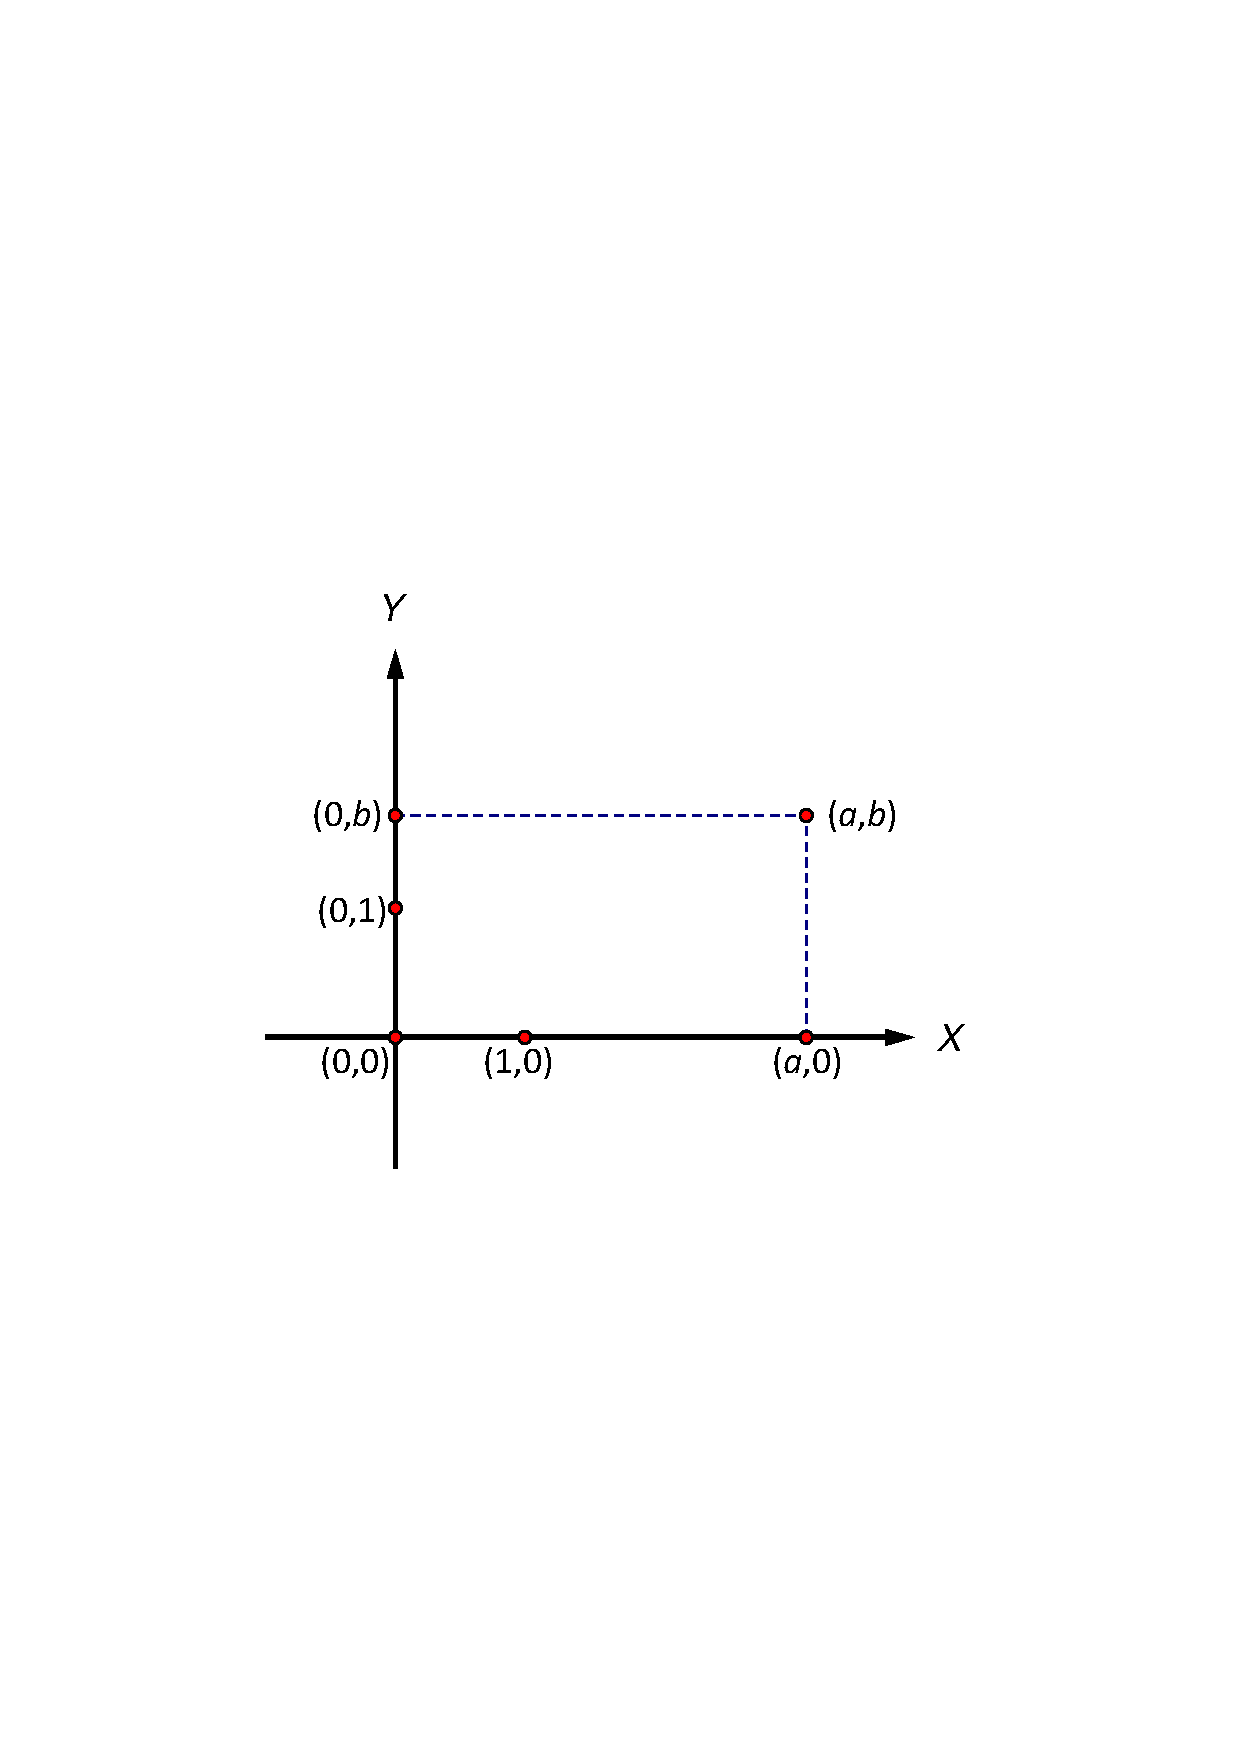
\includegraphics[trim=3cm 9.5cm 3cm 9.5cm,width=0.5\textwidth,clip]{Geometer/KompleksPlan1.pdf}\\
Figur 29.1: Seks komplekse tal i $(x,y)$-planen.		
\end{center}

Vi vil nu ændre skrivemåden for de komplekse tal, idet vi indsætter dem i den komplekse talplan hvis førsteakse vi kalder \textit{realaksen} og andenakse for \textit{imaginæraksen}. Ændringen gennemføres således:
\begin{enumerate}
\item
Alle komplekse tal af typen $(a,0)$, det vil sige de tal der ligger på realaksen, skrives som $a\,$. 
\item
Det komplekse tal $(0,1)$ skrives som $i\,$. Bogstavet $i$ kaldes den \textit{imaginære} enhed.
\item
Alle komplekse tal af typen $(0,b)$, det vil sige de tal der ligger på imaginæraksen, skrives som $i\cdot b$ eller alternativt $b\cdot i$. Ofte udelades gangetegnet, så der blot skrives $ib$ eller $bi$. Hvis $b=0\,$, er $ib=0\,$. 
\item
Alle komplekse tal af typen $(a,b)$ skrives som $a+i\cdot b$ eller alternativt $a+b\cdot i\,$. Også her kan gangetegnet udelades.
\end{enumerate}
På figur 29.2 ses en opdatering af situationen fra figur 29.1 med de nævnte ændringer.

\begin{center}
	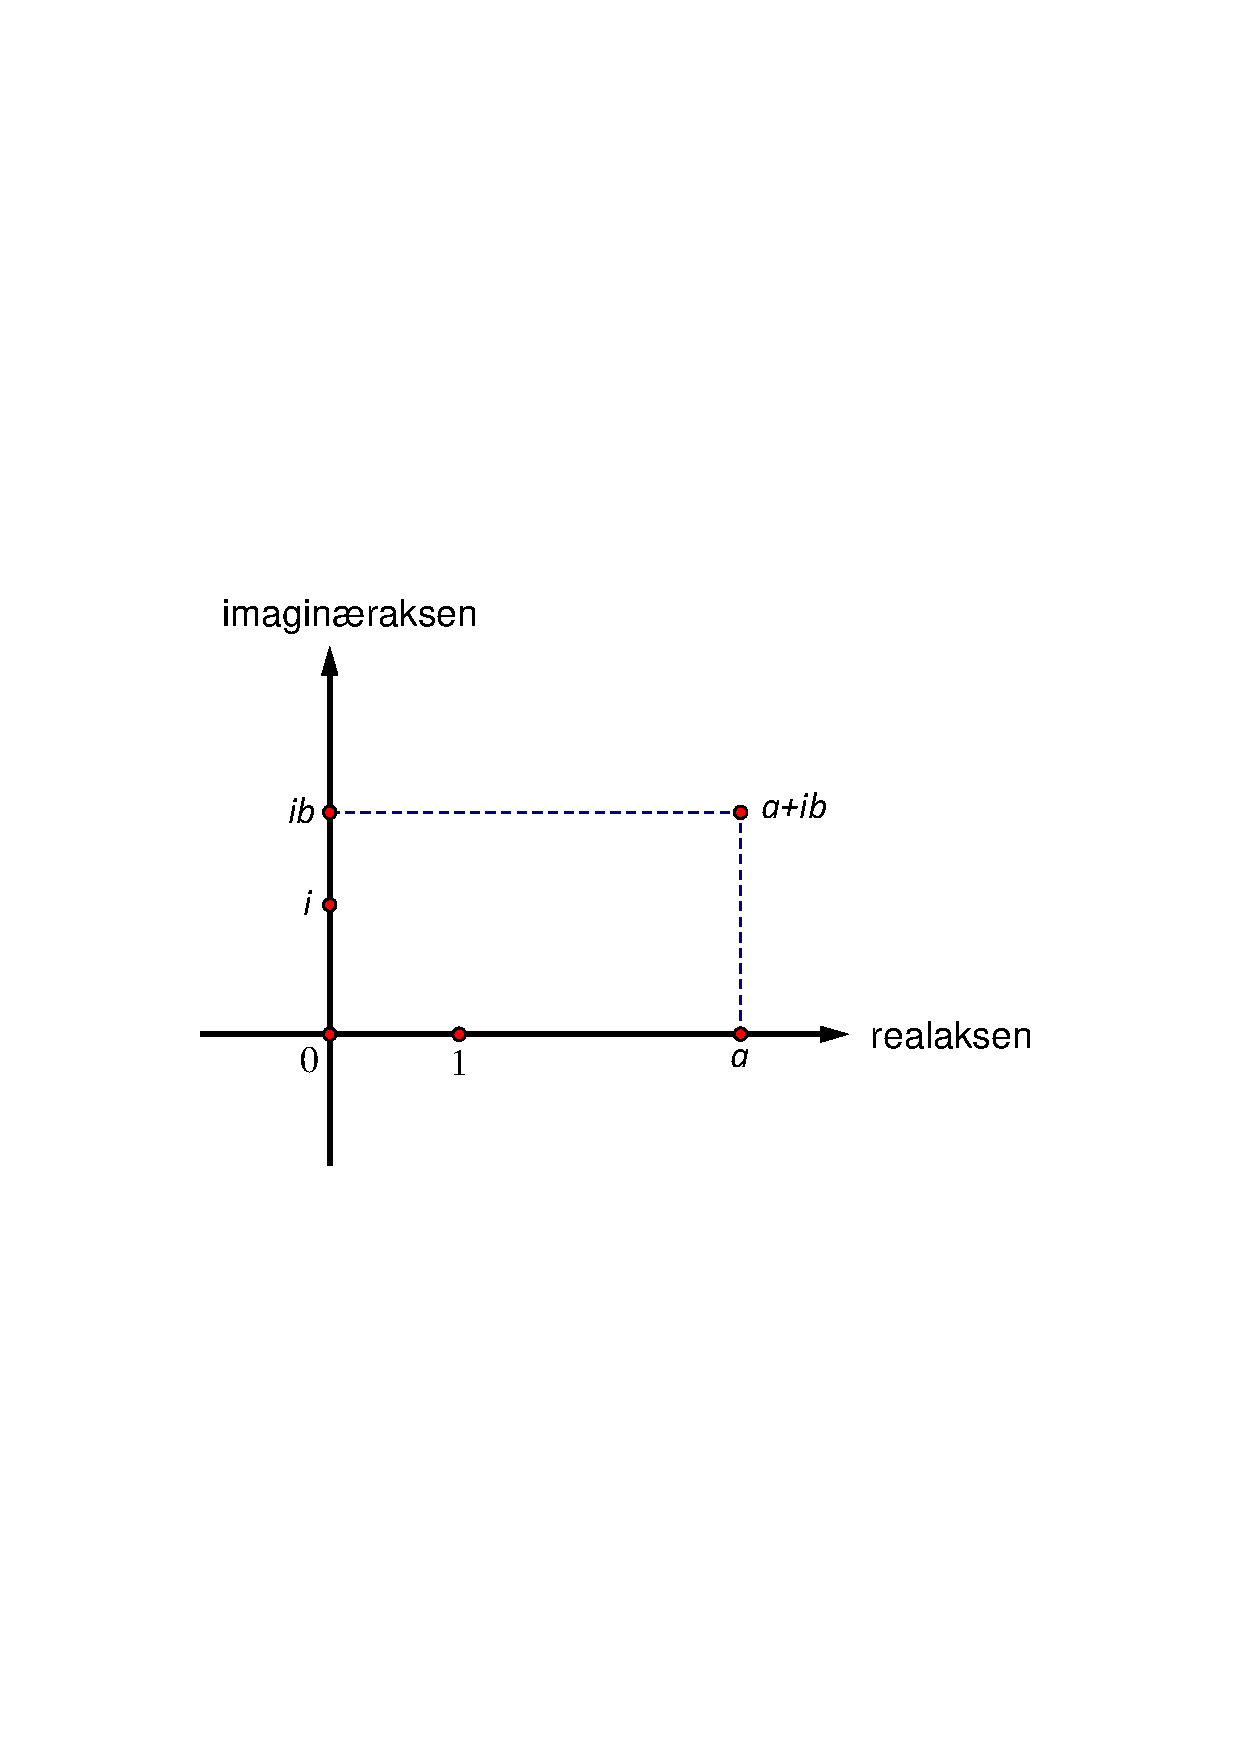
\includegraphics[trim=3cm 9.5cm 3cm 9.5cm,width=0.5\textwidth,clip]{Geometer/KompleksPlan2.pdf}\\
Figur 29.2: Seks komplekse tal i den komplekse talplan.		
\end{center}

\begin{definition}[Komplekse tals rektangulære form]
Ved et komplekst tal $z$ forstås et talpar $(a,b)\in \reel^2$. Mængden af komplekse tal betegnes $\mathbb C\,.$\bs
Det komplekse tal $(0,1)$ tildeles symbolet $i$.\bs Standardskrivemåden for det komplekse tal $z=(a,b)$ er 
 $z=a+ib$ eller alternativt $z=a+bi$. Den kaldes det komplekse tals \textit{rektangulære} form.\bs
Bemærk følgende forkortede skrivemåder: $(a,0)$ skrives blot som $a$ og $(0,b)$ som $ib=bi$. Endvidere: $0i=i0=0\,,\,1i=i1=i\,,\,(-1)i=i(-1)=-i$ og for $k>0:$ $(-k)i=i(-k)=-ik=-ki\,$.
\end{definition}

\begin{aha}
To komplekse tal $z_1=a_1+ib_1$ og $z_2=a_2+ib_2$ kaldes ens hvis $a_1=a_2$ og $b_1=b_2\,$, og vi skriver i så fald $z_1=z_2\,$. 
\end{aha}


\begin{example}[Den komplekse talplan]
Vi indsætter de komplekse tal $-2,\,0,\,1,\,i,\,2-i,\,1+2i,-2+3i$ og $-1-2i$ i den komplekse talplan:
\begin{center}
	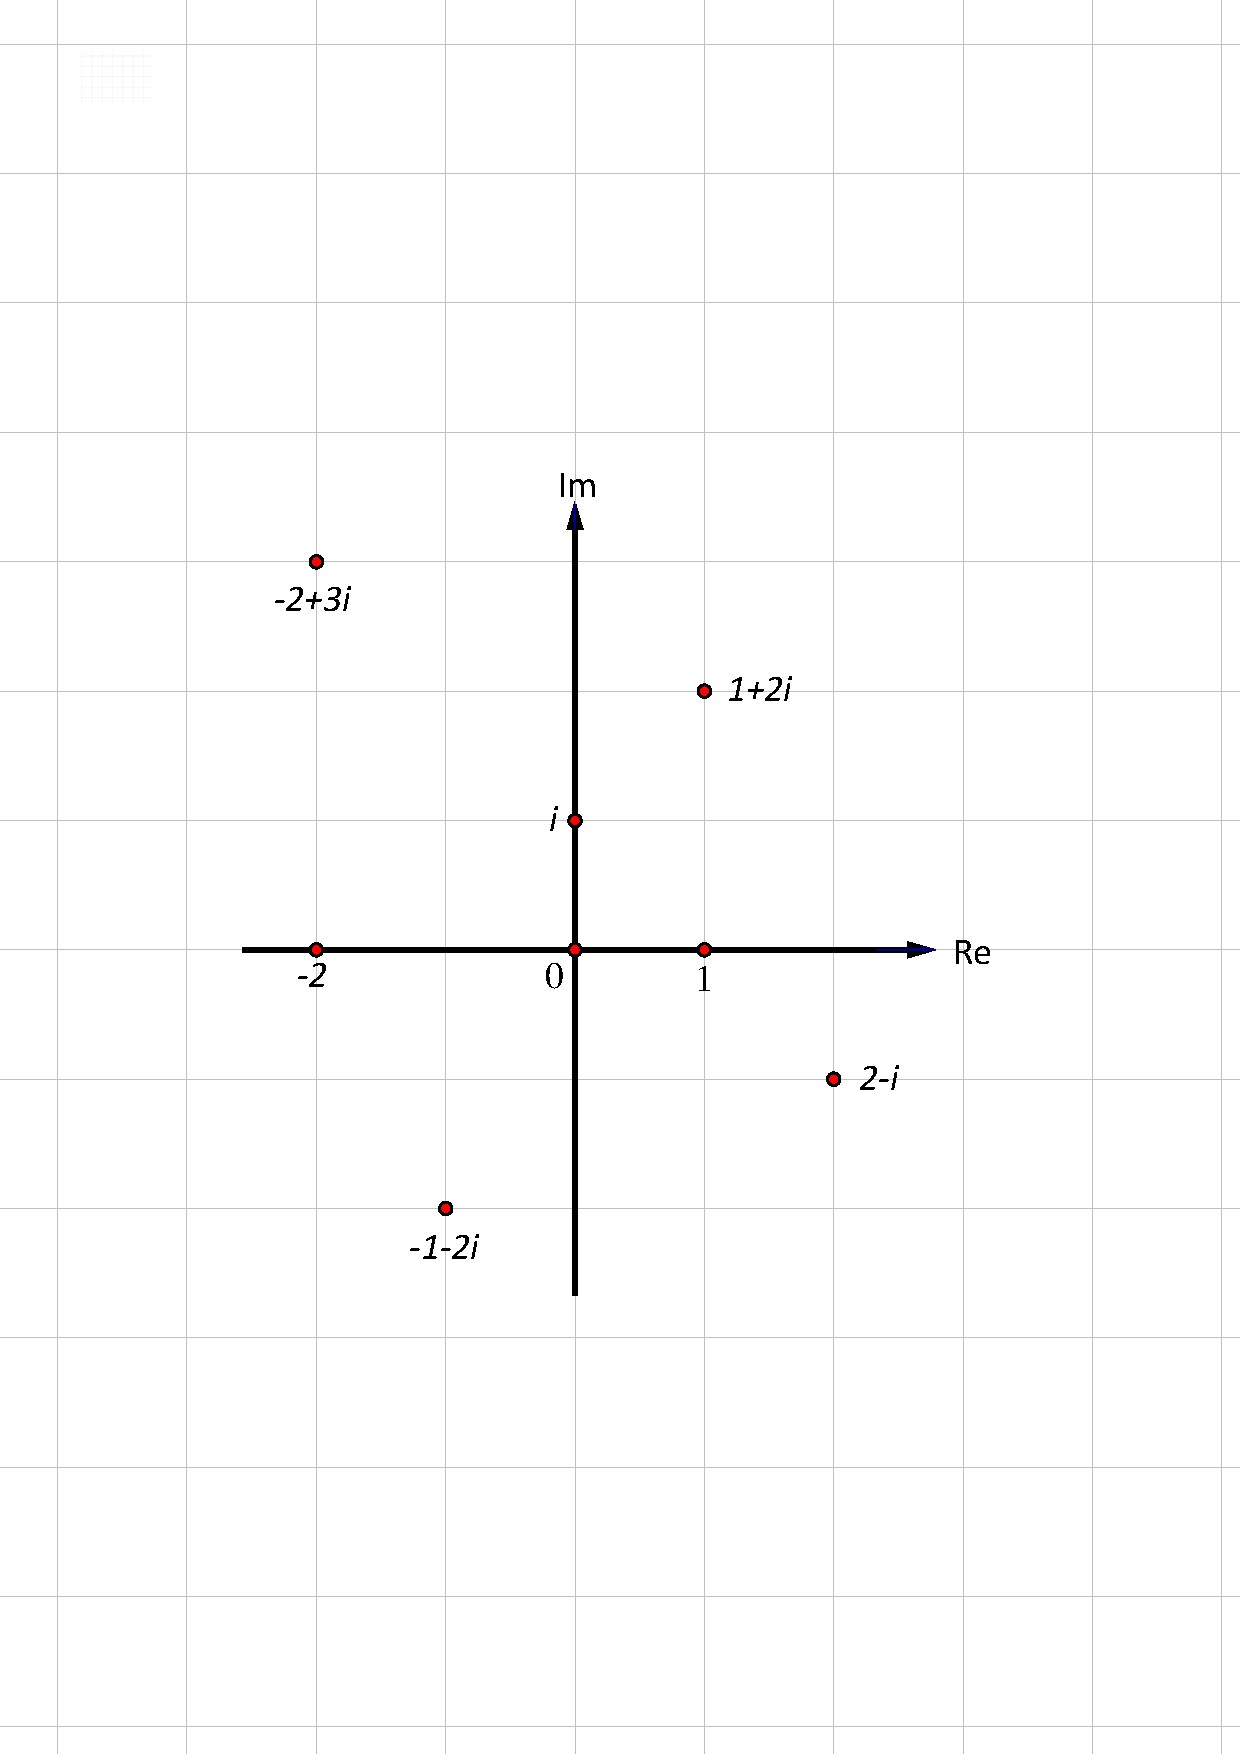
\includegraphics[trim=3cm 8cm 3cm 8cm,width=0.5\textwidth,clip]{Geometer/KompleksPlan3.pdf}\\
Figur 29.3: Eksempler på komplekse tal 
\end{center}
\end{example}

\begin{definition}[Realdel og Imaginærdel]
 
Ved \textit{realdelen} af det komplekse tal $z=(a,b)$ forstås det reelle tal
\begin{equation}
\mathrm{Re}(z)=\mathrm{Re}(a+ib)=a\,, 
\end{equation}
og ved \textit{imaginærdelen} forstås det reelle tal
\begin{equation}
\mathrm{Im}(z)=\mathrm{Im}(a+ib)=b\,.
\end{equation}
\end{definition}

\begin{aha}
Ethvert komplekst tal $z$ kan opskrives på rektangulær form således
$$z=\mathrm{Re}(z)+i\mathrm{Im}(z)\,.$$
\end{aha}

\begin{example}[Realværdi og Imaginærværdi]

Tre komplekse tal er givet ved:
$$z_1=3-2i\,,\,\,z_2=i5\,,\, z_3=25+i\,.$$
Vi finder realdelen og imaginærdelen af tallene:
\begin{equation}
\mathrm{Re}(z_1)=3\,,\,\mathrm{Im}(z_1)=-2\,,\,
\mathrm{Re}(z_2)=0\,,\,\mathrm{Im}(z_2)=5\,,\,
\mathrm{Re}(z_3)=25\,,\,\mathrm{Im}(z_3)=1\,.
\end{equation}
\end{example}

\section{Regning med komplekse tal}
Det karakteristiske ved de størrelser vi kalder tal, er at vi kan regne med dem i over\-ensstemmelse
med de fire klassiske regningsarter (addition, subtraktion, multiplikation og division).
Vi må derfor definere disse regningsarter for de komplekse tal og starter med at indføre
sum og differens.
 
\begin{definition}[Sum og differens af komplekse tal]\label{tn29_sum}
Lad $z_1=a+ib$ og $z_2=c+id,$ hvor $a,b,c$ og $d$ er reelle tal.\bs
Summen $z_1+z_2$ defineres ved
\begin{equation}\label{tn29_sum1}
z_1+z_2=(a+c)+i(b+d)\,.
\end{equation}
Differensen $z_1-z_2$ defineres ved
\begin{equation}\label{tn29_sum2}
z_1-z_2=(a-c)+i(b-d)\,.
\end{equation}
\end{definition}
\begin{aha}
En stor fordel ved $a+ib$ formen af komplekse tal er at man ikke behøver huske formlerne i definition \ref{tn29_sum}! Men kan nemlig addere og subtrahere komplekse tal på samme måde som reelle tal, når blot $i$ behandles efter de samme regler som ville gælde en reel konstant. Den indførte sum kan nemlig udregnes ved ''sædvanlige'' regneregler således:
$$z_1+z_2=(a+ib)+(c+id)=(a+c)+(ib+id)=(a+c)+i(b+d),$$
og den indførte differens tilsvarende:
$$z_1-z_2=(a+ib)-(c+id)=(a-c)+(ib-id)=(a-c)+i(b-d)\,.$$
\end{aha}
\begin{example}
Det bemærkes at addition og subtraktion i den komplekse talplan svarer til addition og subtraktion af vektorer i planen. I figur 29.4 er et eksempel på addition ved parallelogram-metoden:
\begin{center}
	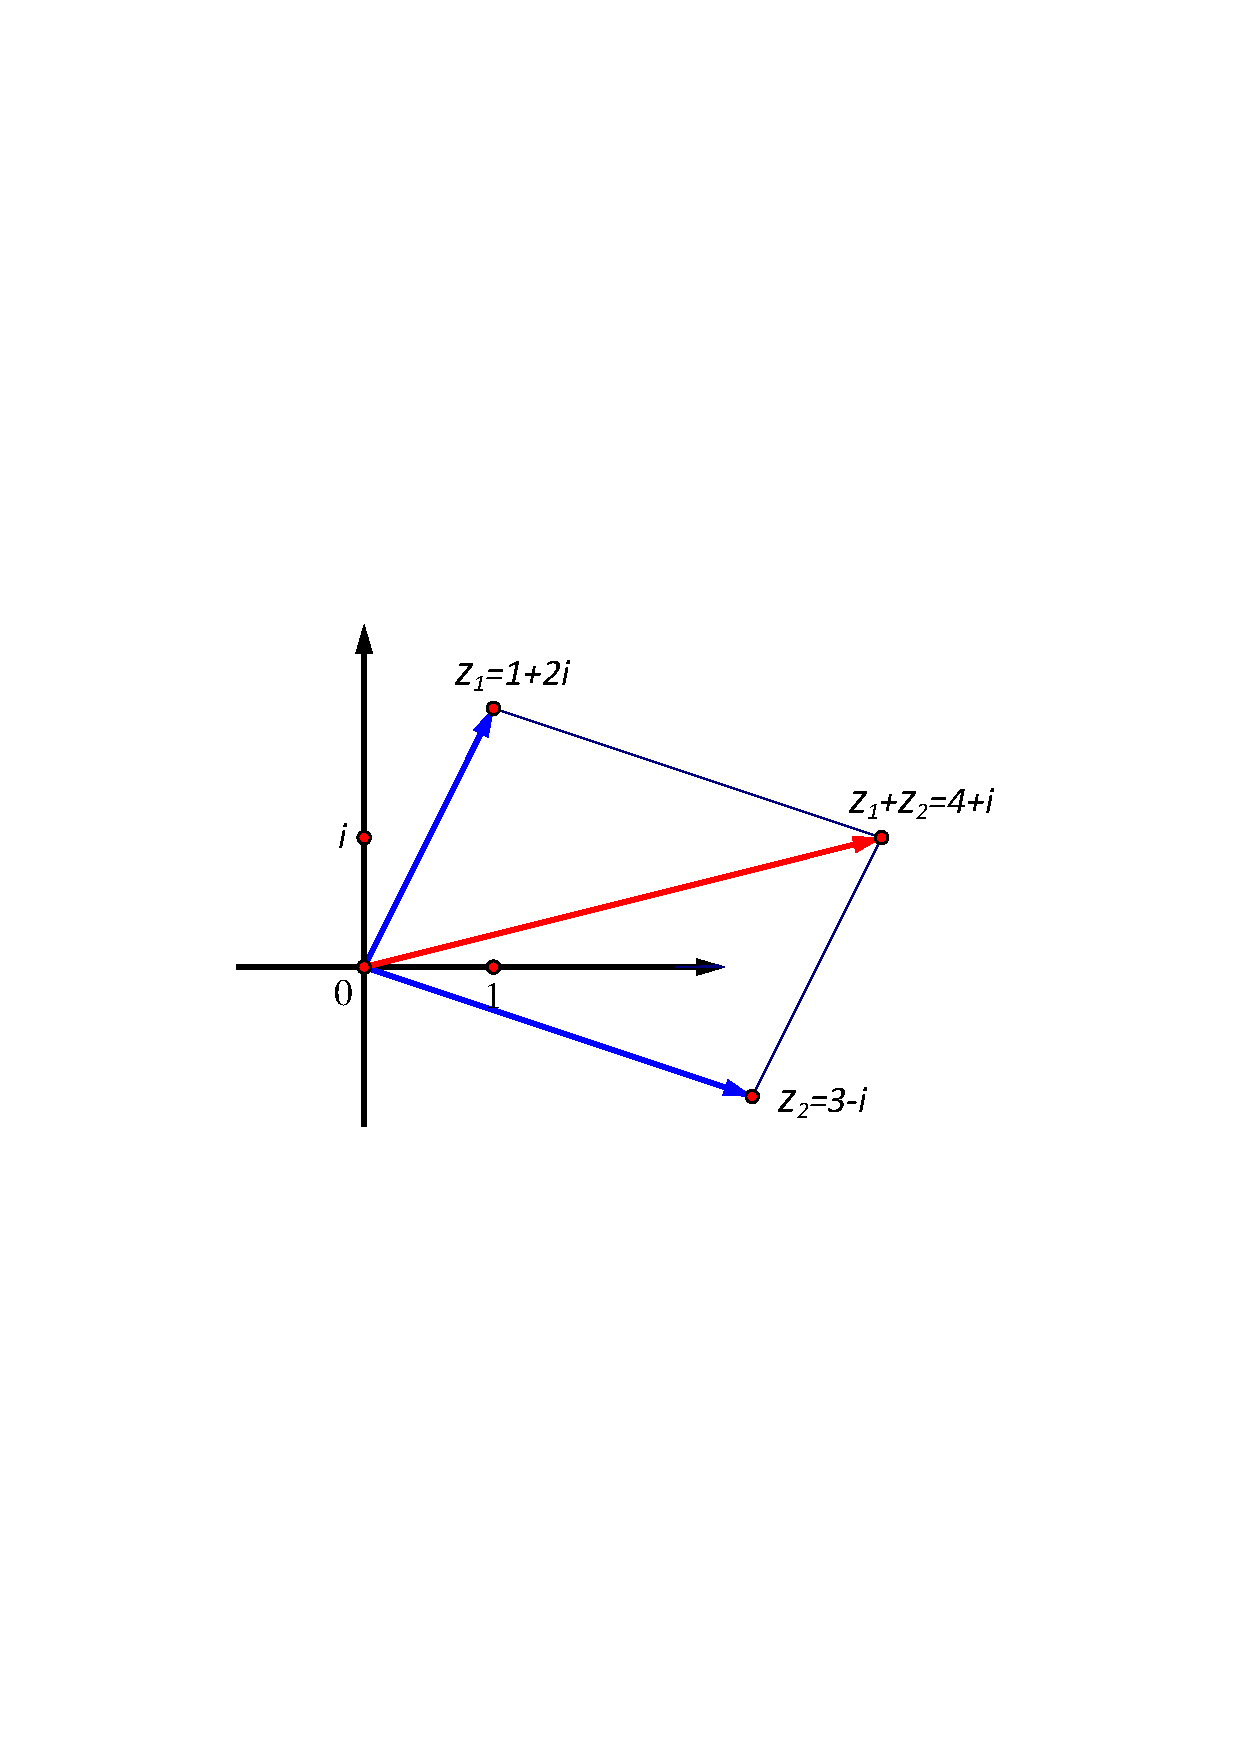
\includegraphics[trim=3cm 9cm 3cm 10cm,width=0.5\textwidth,clip]{Geometer/KompleksPlan4.pdf}\\
Figur 29.4: Addition ved parallelogram-metoden 
\end{center}
\end{example}


\begin{definition}[Multiplikation af komplekse tal]\label{tn29_produkt}
Vi definerer først kvadratet på den imaginære enhed $i\,$:
$$i^2=i\cdot i =-1\,.$$
Lad $z_1=a+ib$ og $z_2=c+id$.\bs
Produktet $z_1\,z_2$ defineres ved
\begin{equation}\label{tn29_produkt1}
z_1\,z_2=z_1\cdot z_2= (ac-bd)+i(ad+bc)\,.
\end{equation}
\end{definition}
\begin{aha}
Bemærk at man strengt taget ikke behøver huske formel (\ref{tn29_produkt1}). Vi kan  multiplicere  komplekse tal på samme måde som reelle tal, når blot $i$ behandles efter de samme regler som ville gælde en reel konstant, og det huskes at $i^2=-1$. Det indførte produkt kan nemlig udregnes ved ''sædvanlige'' regneregler således:
$$z_1z_2=(a+ib)(c+id)=ac+iad+ibc+i^2bd$$
$$=(ac-bd)+i(ad+bc)\,.$$
\end{aha}

\begin{definition}[Division af komplekse tal]\label{tn29_broek}
Lad $z_1=a+ib$ og $z_2=c+id\,$, hvor ikke både $c$ og $d$ er lig med $0$.\bs
Brøken $\,\displaystyle{\frac{z_1}{z_2}}\,$ defineres ved 
\begin{equation}\label{tn29_broek1}
\frac{z_1}{z_2}=\frac{ac+bd}{c^2+d^2}+i\,\frac{bc-ad}{c^2+d^2}\,.
\end{equation}
\end{definition}

\begin{aha}
Heller ikke ved division behøver man huske formlen.  Division af komplekse tal kan udføres ved hjælp af ``sædvanlige'' regneregler for reelle tal, når blot $i$ behandles efter de samme regler som ville gælde en reel konstant, og det huskes at $i^2=-1$. Den indførte division (\ref{tn29_broek1}) kan nemlig udregnes således:\\
$$\frac{z_1}{z_2}=\frac{a+ib}{c+id}
=\frac{(a+ib)(c-id)}{(c+id)(c-id)}$$
$$=\frac{(ac+bd)+i(bc-ad)}{c^2+d^2}
=\frac{ac+bd}{c^2+d^2}+i\,\frac{bc-ad}{c^2+d^2}\,.$$
\end{aha}

Efter indføringen af de fire sædvanlige regnearter for komplekse tal, kan vi nu præcisere sammenhængen mellem de reelle tal og de komplekse. Da vi har valgt at skrive tal på formen $a+i0$ som $a\,$, ligner alle de komplekse tal der ligger på realaksen, almindelige reelle tal. Realaksen er simpelthen en almindelig reel talakse. De regnearter vi har indført for komplekse tal, stemmer for alle tal på realaksen overens med de sædvanlige regnearter for reelle tal. Lad os eksemplificere dette med multiplikation.\bs
To komplekse tal er på rektangulær form givet ved $a$ og $c\,$. Vi udregner deres produkt ved hjælp af (\ref{tn29_produkt1}):
$$
a\cdot c=(a+i\cdot0)(c+i\cdot0)=(a\cdot c-0\cdot0)+i(a\cdot0+0\cdot c)=a\cdot c+i\cdot0=a\cdot c\,.
$$
På tilsvarende vis vises at de indførte definitioner på kompleks addition, subtraktion og division på realaksen stemmer overens med de reelle.\bs
Derfor kan de komplekse tal betragtes som en \textit{udvidelse} eller \textit{generalisering} af de reelle tal.


\section{Polære koordinater}
Den oplagte måde at angive et punkt i et sædvanligt
$(x,y)$-koordinatsystem på, er naturligvis punktets retvinklede koordinater. I mange situationer er det imidlertid nyttigt at kunne bestemme et punkt ved dets \textit{polære koordinater}, som består af punktets afstand til Origo samt punktets \textit{retningsvinkel} fra $x$-aksen til forbindelseslinjen mellem Origo og punktet, idet den regnes positiv hvis den udmåles mod uret, og negativ hvis den udmåles med uret.\bs

I det følgende indfører vi på tilsvarende vis polære koordinater for komplekse tal. Lad os først præcisere en orientering af den komplekse talplan:

\begin{definition}[Orientering af den komplekse talplan]
Orientering af den komplekse talplan fastlægges ved at en cirkel med centrum i tallet $0$ gennemløbes \textit{mod uret}.
\begin{center}
	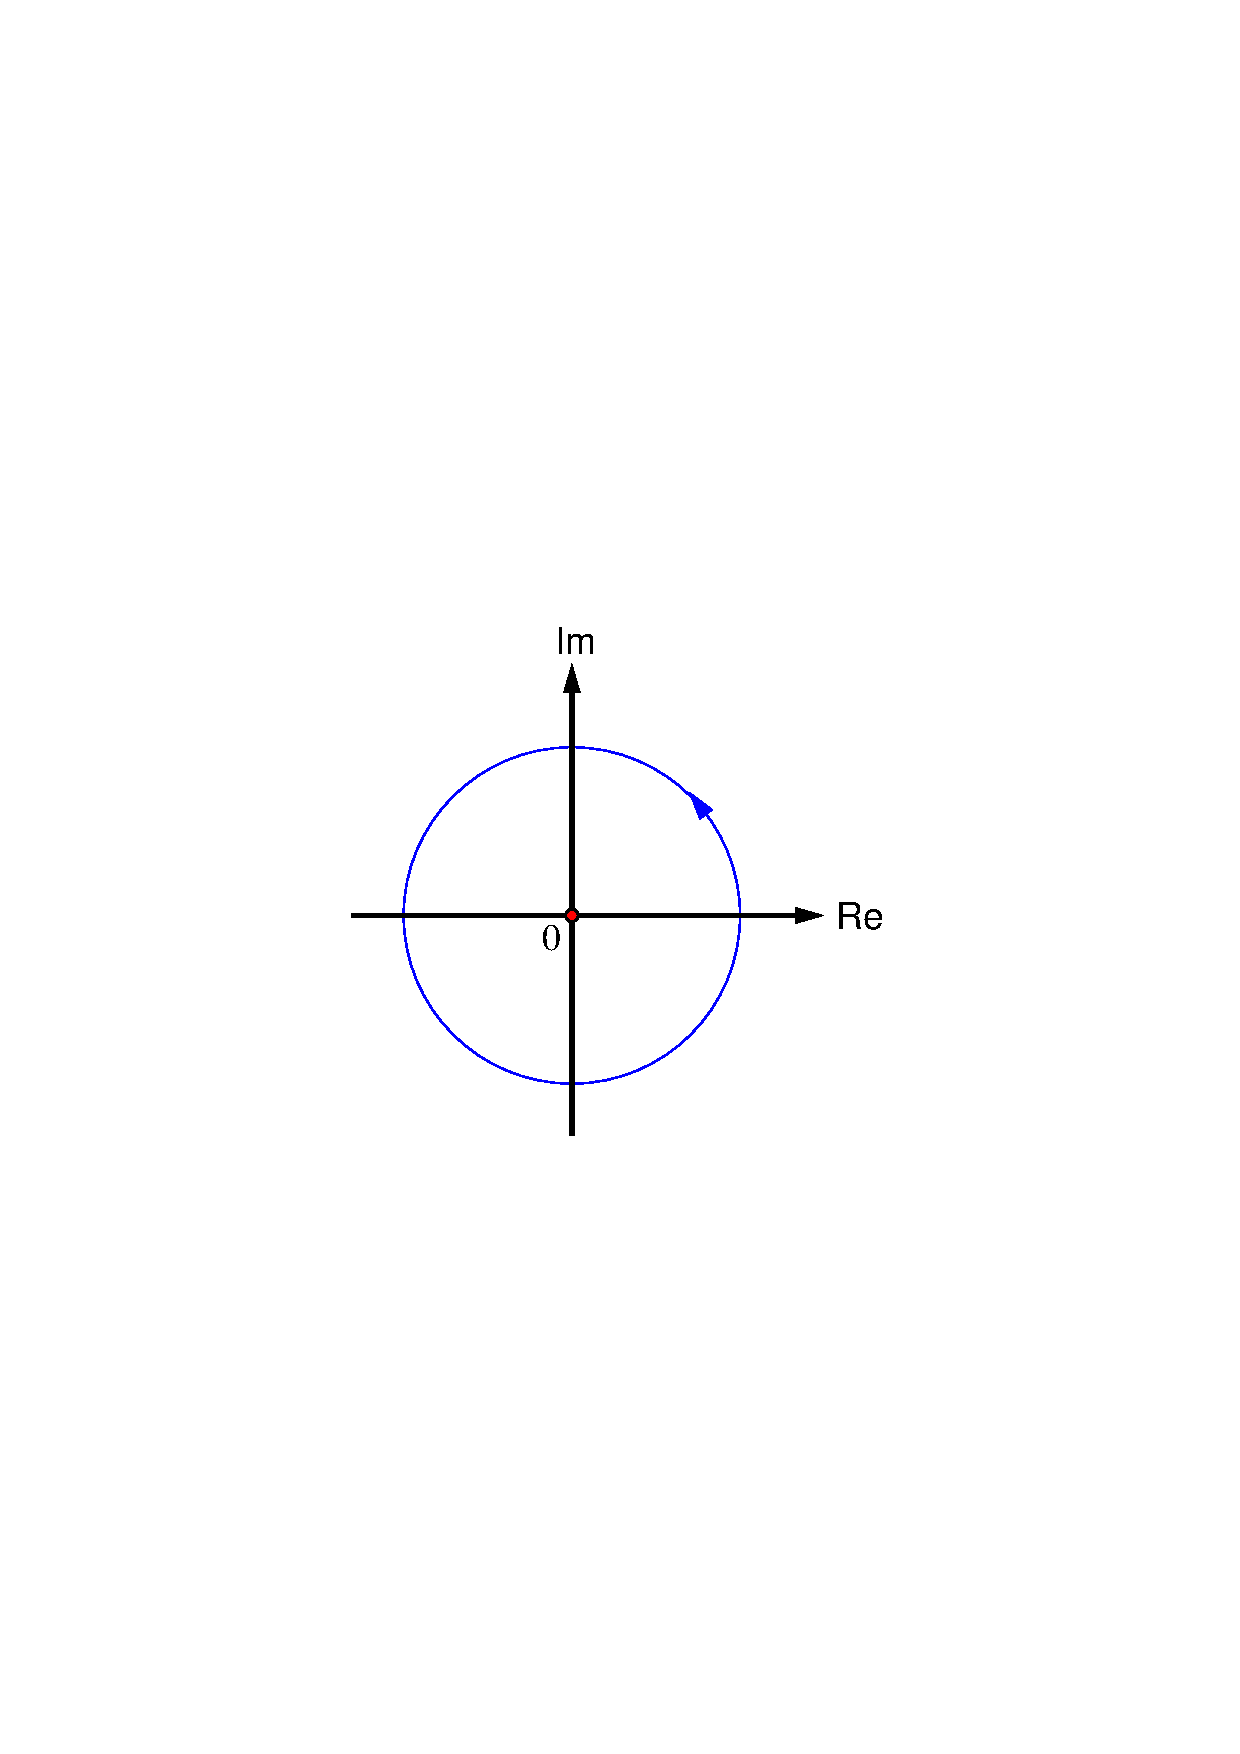
\includegraphics[trim=3cm 10.8cm 3cm 10.6cm,width=0.44\textwidth,clip]{Geometer/orientering.pdf}\\
Figur 29.5: Den komplekse talplans orientering		
\end{center}
\end{definition}

Ingredienserne i polære koordinater for et komplekst tal er tallets absolutværdi og tallets argument. Dem indfører vi nu.

\begin{definition}[Absolutværdi og argument]
Givet et komplekst tal $z\,$.\bs 
Ved \textit{absolutværdien} af $z$ forstås afstanden fra Origo til $z\,$. Absolutværdien skrives $|\,z\,|$ og kaldes også for $z$'s \textit{modulus} eller \textit{numeriske værdi}.\bs
Antag $z\neq 0\,$. Enhver vinkel fra realaksens positive del til forbindelseslinjen mellem Origo og $z$ kaldes et \textit{argument} for $z$ og betegnes arg$(z)\,$. Vinklen regnes med fortegn i overensstemmelse med orienteringen af den komplekse talplan.
\begin{center}
	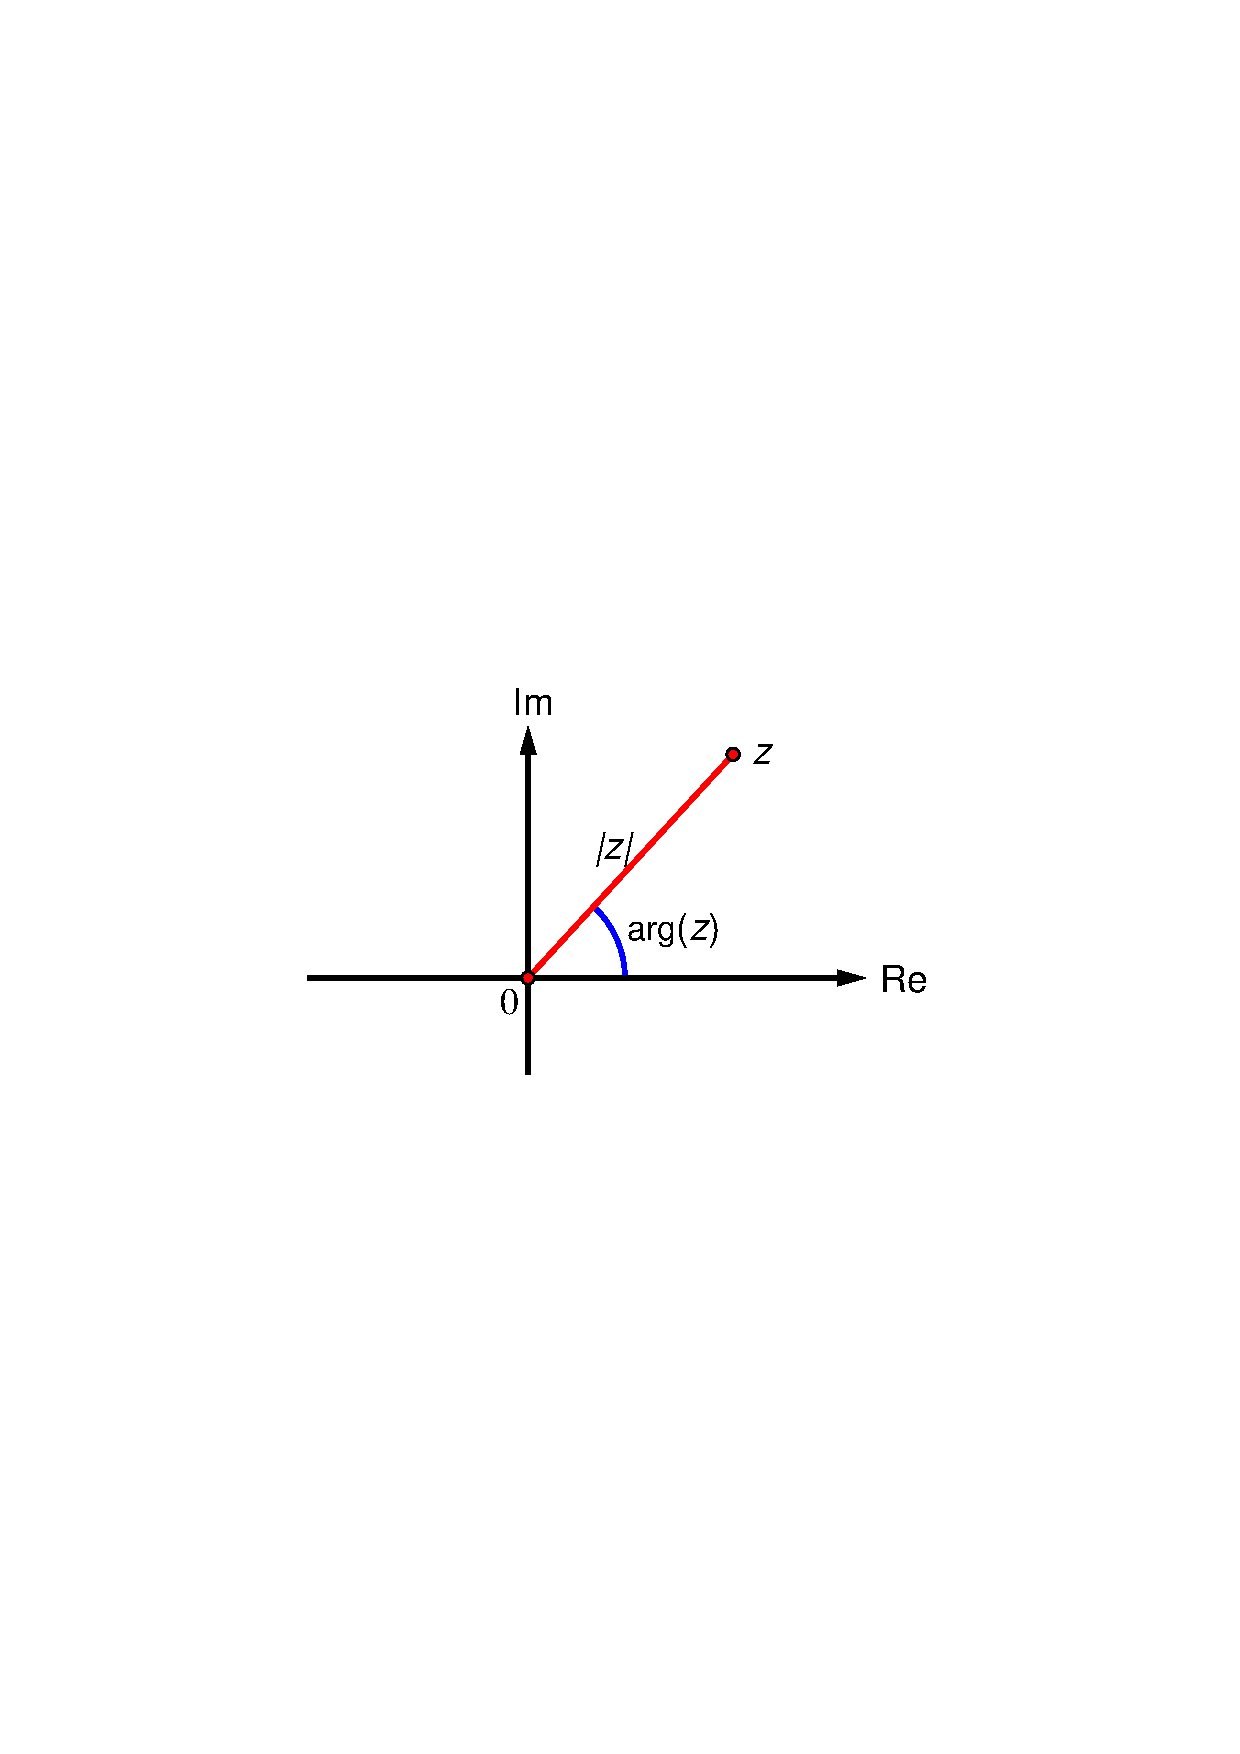
\includegraphics[trim=3cm 12cm 3cm 11.5cm,width=0.5\textwidth,clip]{Geometer/polar.pdf}\\
Figur 29.6: Absolutværdi og argument
\end{center}
Et sammenhørende par $$\big(\,|\,z\,|\,,\mathrm{arg}(z)\,\big )$$ af absolutværdien af $z$ og et argument for $z$  kaldes for \textit{polære koordinater} for $z\,$.
\end{definition}

Bemærk at argumentet for et tal $z$ ikke er entydigt. Hvis man for eksempel til et valgt\- argument for $z$ lægger vinklen $2\pi\,$, opnår man igen en gyldig retningsvinkel for halvlinjen fra $0$ til $z$ og dermed et nyt argument for tallet. Således ses at $z$ har uendeligt mange argumenter.\bs
Man kan imidlertid altid vælge et argument for $z$ som ligger i intervallet fra $-\pi$ til $\pi$. Der er tradition for at give dette argument en fortrinsstilling, det kaldes for tallets ho\-vedargument.\bs
\begin{definition}[Hovedargument]
Ved \textit{hovedargumentet} for $z\in \mathbb C\,$ betegnet Arg$(z)$ forstås det entydigt bestemte argument for $z$ som opfylder
$$\mathrm{Arg}(z)\in\mathrm{]}-\pi,\pi\,\mathrm{]}\,.$$
\end{definition}
Det ses at samtlige argumenter for $z$ kan fastlægges ved 
\begin{equation}
\arg(z)=\mathrm{Arg}(z)+p\cdot 2\pi\,\,,\,p\in \mathbb Z\,.
\end{equation}
\begin{example}[Hovedargumenter]

\begin{center}
	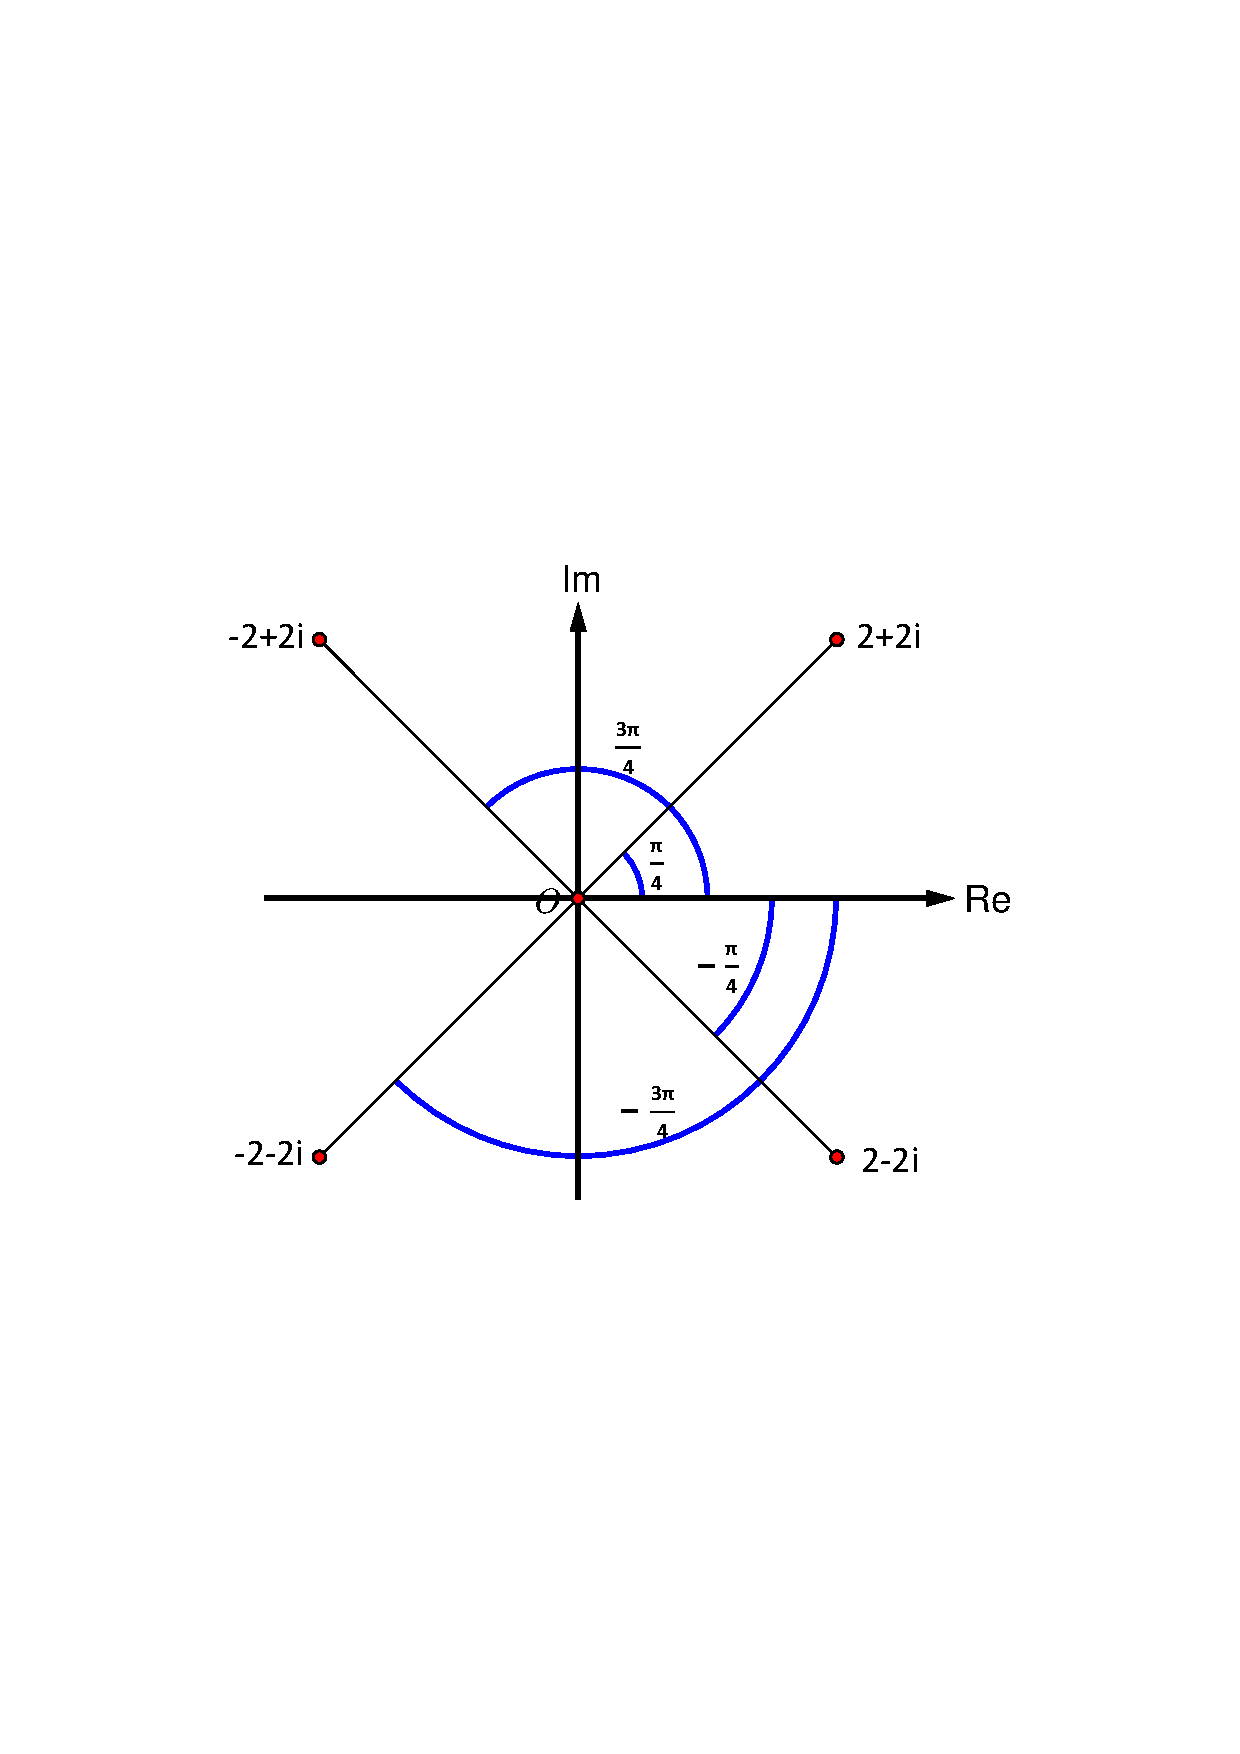
\includegraphics[trim=3cm 8.5cm 3cm 9.5cm,width=0.55\textwidth,clip]{Geometer/retningsvinkel2.pdf}\\
Figur 29.7: Hovedargumenter
\end{center}
%Ved brug af Pythagoras fås at alle de fire angivne tal har absolutværdien $\sqrt{2}\,$.
På figuren er angivet fire komplekse tal som ligger på vinkelhalveringslinjer mellem akserne. Deres hovedargumenter aflæses umiddelbart: $2+2i$ har hovedargumentet $\frac {\pi}4\,$, $2-2i$ har hovedargumentet $-\frac {\pi}4\,$, $-2+2i$ har hovedargumentet $\frac {3\pi}4\,$, og endelig har $-2-2i$ ho\-ved\-argumentet $-\frac {3\pi}4\,$.
\end{example}

 
Vi har nu to forskellige fremgangsmåder til rådighed
til beskrivelse af komplekse tal. Et komplekst tal kan angives på rektangulær form eller ved hjælp af dets polære koordinater. I metode \ref{tn29_omform} demonstreres det hvordan man kan veksle mellem de to fremgangsmåder. 

\begin{method}[Rektangulære og polær koordinater]\label{tn29_omform}
Vi betragter et komplekst tal $z\neq 0$ med rektangulær form $z=a+ib$. Antag videre at $z$ har absolutværdien $|\,z\,|=r$ og et argument arg$(z)=v\,$: 
\begin{center}
	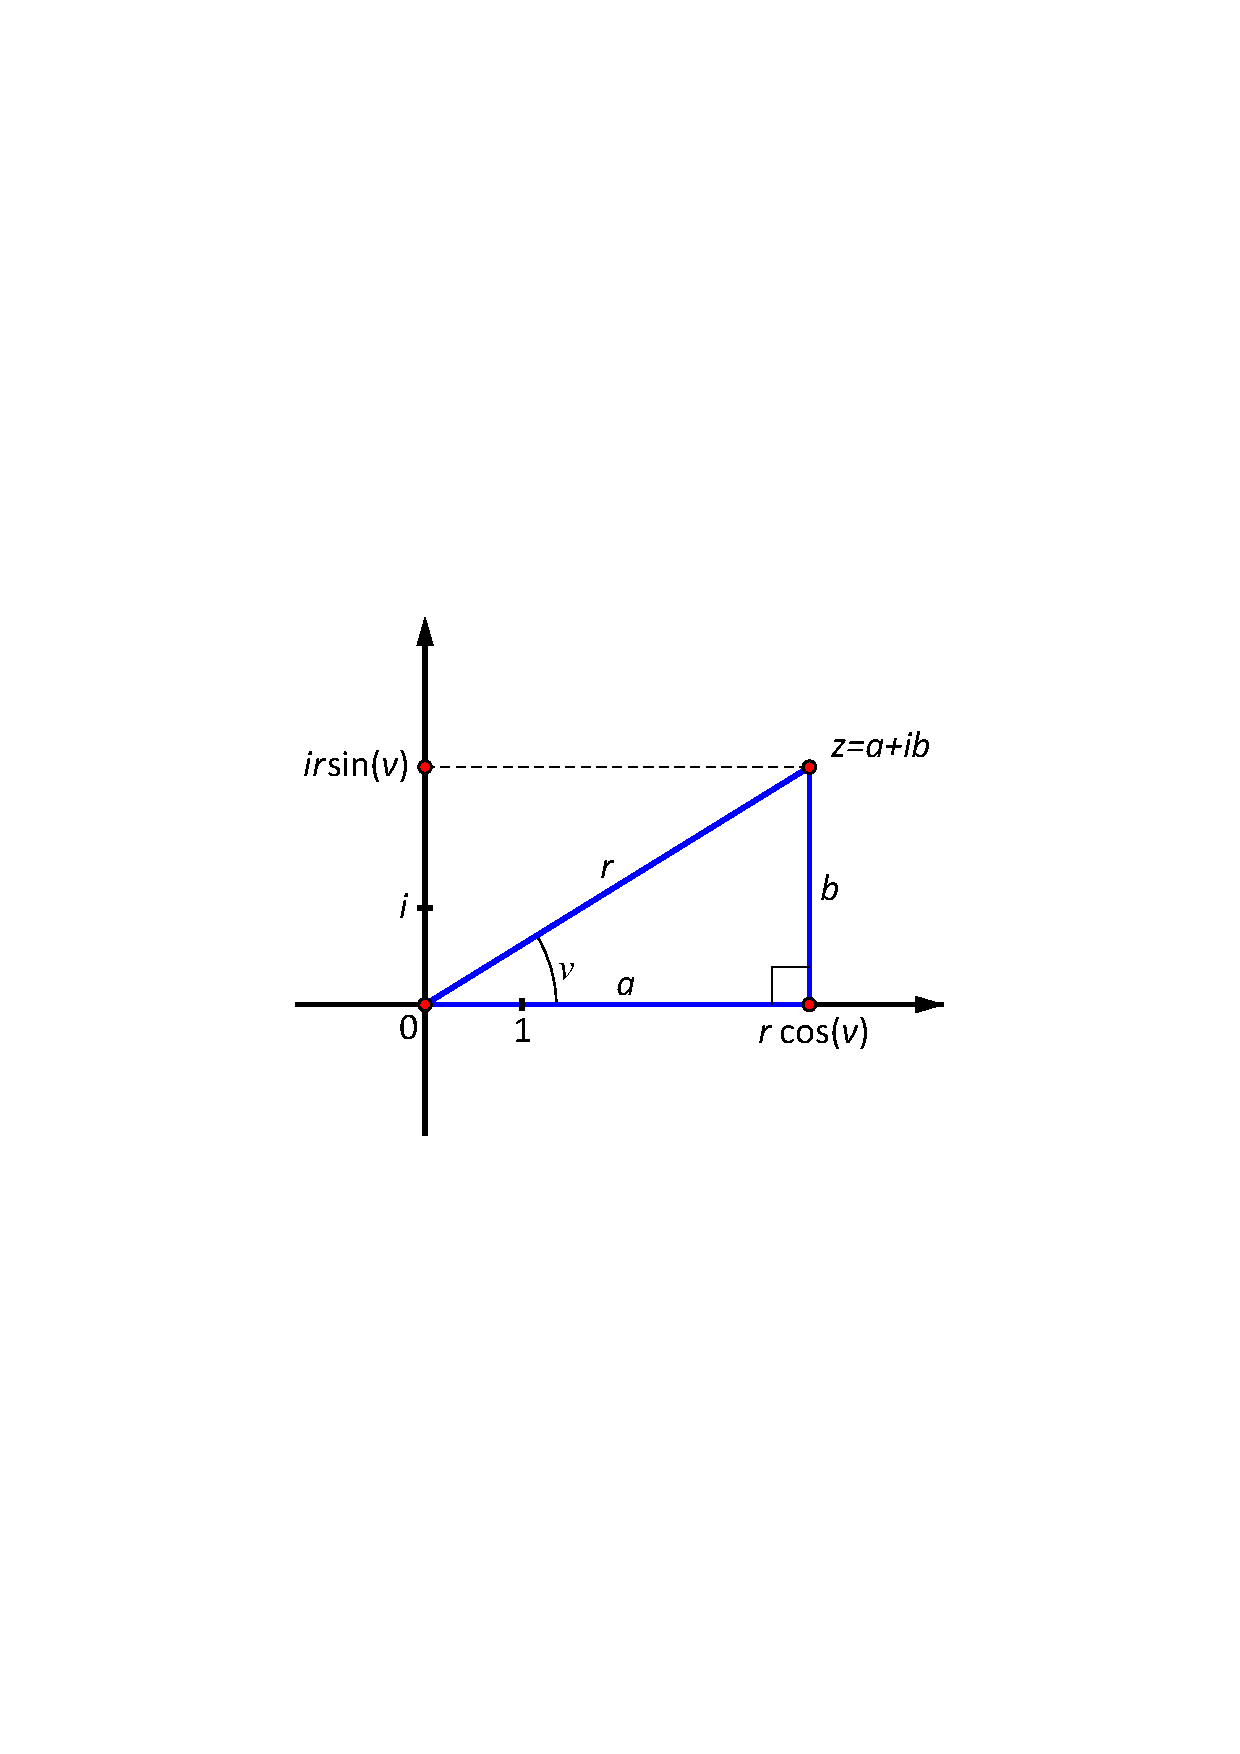
\includegraphics[trim=3cm 10.5cm 3cm 10.5cm,width=0.6\textwidth,clip]{Geometer/omformning1.pdf}\\
Figur 29.8: Omformning af koordinater
\end{center}
\begin{enumerate}
\item
Rektangulær form fås ud fra de polære koordinater således:
\begin{equation}\label{tn29_omform1}
a=r\cos(v)\,\,\,\mathrm{og}\,\,\,b=r\sin(v)\,.
\end{equation}
\item
Absolutværdien fås ud fra den rektangulære form således:
\begin{equation}\label{tn29_omform2}
r=\sqrt{a^2+b^2}\,.
\end{equation}
\item
Et argument fås ud fra den rektangulære form således:
\begin{equation}\label{tn29_omform3}
\cos(v)=\frac a r \,\,\,\mathrm{og}\,\,\,\sin(v)=\frac b r\,. 
\end{equation}
\end{enumerate}
\end{method}
\begin{aha}
NB: Når $z$ som på figuren i metode \ref{tn29_omform} er tegnet i 1. kvadrant, er det oplagt at regel (\ref{tn29_omform1}) og (\ref{tn29_omform3}) kommer fra velkendte sætninger om cosinus og sinus til spidse vinkler i retvinklede trekanter og (\ref{tn29_omform2}) fra Pythagoras' sætning. Med de samme sætninger kan det vises at de indførte metoder gælder uanset hvilken kvadrant $z$ ligger i. 
\end{aha}

\begin{example}[Fra rektangulær til polær form]\label{tn29_exOmform}
Vi vil finde de polære koordinater for tallet $z=-\sqrt 3+i\,$ ved hjælp af metode \ref{tn29_omform}.
\begin{center}
	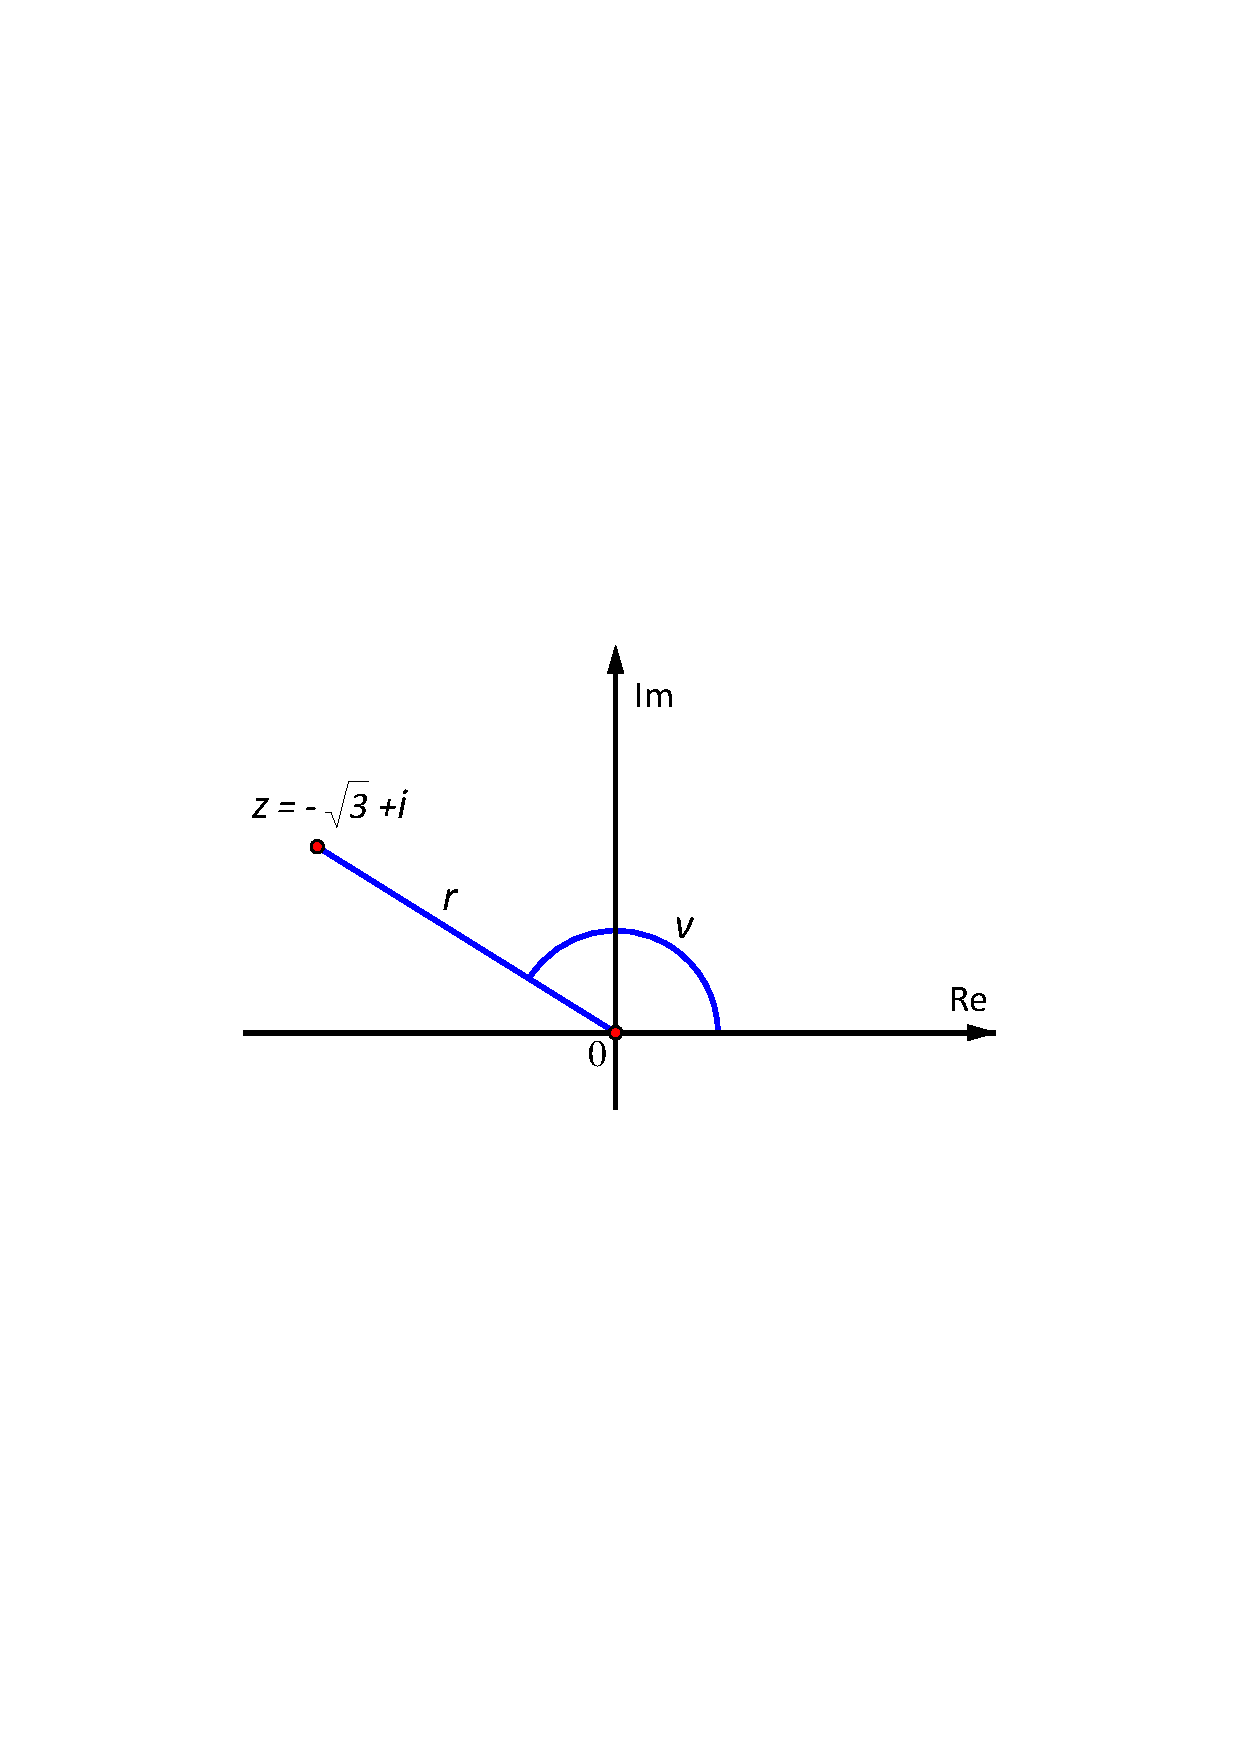
\includegraphics[trim=3cm 11cm 3cm 11cm,width=0.5\textwidth,clip]{Geometer/omformning3.pdf}\\
Figur 29.9: Bestemme polære koordinater 
\end{center}

Vi bestemmer først absolutværdien:
$$
r=|\,z\,|=\sqrt{(-\sqrt 3)\,^2+1^2}=\sqrt{3+1}=2\,.
$$
Ud fra ligningen
$$\cos(v)=-\frac{\sqrt 3}2$$
får vi to bud på et hovedargument for $z\,$, nemlig
$$v=\frac{5\pi}6\,\,\,\mathrm{og}\,\,\,v=-\frac{5\pi}6\,.$$
På figuren kan vi aflæse at figuren ligger i 2. kvadrant, og at det korrekte hovedargument må være det førstnævnte. Men dette kan også fastlægges uden inspektion af figuren, idet også ligningen
$$\sin(v)=\frac12$$
skal være opfyldt. Fra denne får vi også to bud på et hovedargument for $z\,$, nemlig
$$v=\frac{\pi}6\,\,\,\mathrm{og}\,\,\,v=\frac{5\pi}6\,.$$

Da kun $\begin{displaystyle}v=\frac{5\pi}6\end{displaystyle} $ opfylder begge ligninger, ser vi at $\begin{displaystyle} \mathrm{Arg}(z)=\frac{5\pi}6\,.\end{displaystyle} $\bs

Hermed har vi fundet det polære koordinatsæt for $z\,$:
$$(r,v)=\big(|\,z\,|,\mathrm{Arg}(z)\,\big)=\big(2,\frac{5\pi}6\big)\,.$$
\end{example}

%Ved hjælp af omformingsreglerne i metode \ref{tn29_omform} opnår vi en ny bekvem skriveform for komplekse tal idet vi har:
%$$z=a+ib=r\cos(v)+ir\sin(v)=r\big(\cos(v)+i\sin(v)\big)\,.$$

%\begin{definition}[Trigonometrisk form]
%Ved \textit{trigonometrisk form} for et komplekst tal $z$ med $|\,z\,|=r$ og arg$(z)=v\,$ forstås skrivemåden
%\begin{equation}
%z=r\big(\cos(v)+i\sin(v)\big)\,.
%\end{equation}
%\end{definition}

Multiplikation og division af to komplekse tal på rektangulær form er lidt omstændelig som det fremgår af definition \ref{tn29_produkt}. Og endnu værre bliver det når man skal opløfte komplekse tal til høje potenser. Men hvis man benytter sig af tallenes polære form, viser det sig at disse regnearter bliver overraskende enkle. Til dette får vi brug for regneregler for absolutværdi og argument, regneregler som også er interessante i sig selv. \bs 
\begin{theorem}[Regneregler for absolutværdi]\label{tn29_RegnAbs}
Absolutværdien for produktet af to komplekse tal $z_1$ og $z_2$ fås ved
\begin{equation}\label{tn29_RegnAbs1}
|\,z_1\cdot z_2\,|=|\,z_1\,|\cdot|\,z_2\,|\,.
%\arg(z_1z_2)&=\arg(z_1)+\arg(z_2)
\end{equation}
Absolutværdien for kvotienten af to komplekse tal $z_1$ og $z_2\,$, hvor $z_2\neq 0\,$, fås ved
\begin{equation}\label{tn29_RegnAbs2}
\left|\,\frac{z_1}{z_2}\,\right|=\frac{\left|\,z_1\,\right|}{\left|\,z_2\,\right|}
%\arg(z_1z_2)&=\arg(z_1)+\arg(z_2)
\end{equation}
%Sagt i ord er absolutværdien af et produkt lig med produktet af absolutværdien af hver af faktorerne. Mens et argument for et produktet fås ved summen af et argument for hver af faktorerne.\bs
Absolutværdien af den $n$'te potens af et  komplekst tal $z$ fås ved:
\begin{equation}\label{tn29_RegnAbs3}
|\,{z_1}^n\,|=|\,z_1\,|^n\\
%\arg(z^n)&=n\arg(z)
\end{equation}
\end{theorem}
\begin{bevis}
Med i næste opdatering af eNoten.
\end{bevis}

\begin{theorem}[Regneregler for argumenter]\label{tn29_RegnArg}
Et argument for produktet af to komplekse tal $z_1$ og $z_2$ fås ved
\begin{equation}\label{tn29_RegnArg1}
\arg(z_1\cdot z_2)=\arg(z_1)+\arg(z_2)
\end{equation}
Et argument for kvotienten af to komplekse tal $z_1$ og $z_2$ hvor $z_2\neq 0\,$, fås ved
\begin{equation}\label{tn29_RegnArg2}
\arg\left(\frac{z_1}{z_2}\right)=\arg(z_1)-\arg(z_2)
\end{equation}
Et argument for den $n$'te potens af et  komplekst tal $z$ fås ved:
\begin{equation}\label{tn29_RegnArg3}
\arg(z^n)=n\arg(z)
\end{equation}
\end{theorem}
\begin{bevis}
Med i næste opdatering af eNoten.
\end{bevis}

\begin{example}[Multiplikation vha. polær koordinater]\label{PolarMult}
To komplekse tal $z_1$ og $z_2$ er givet ved de polære koordinater $\big(\frac 12,\frac{\pi}4\,\big)$ henholdsvis $\big(2,\frac{2\pi}3\,\big)\,$.
\begin{center}
	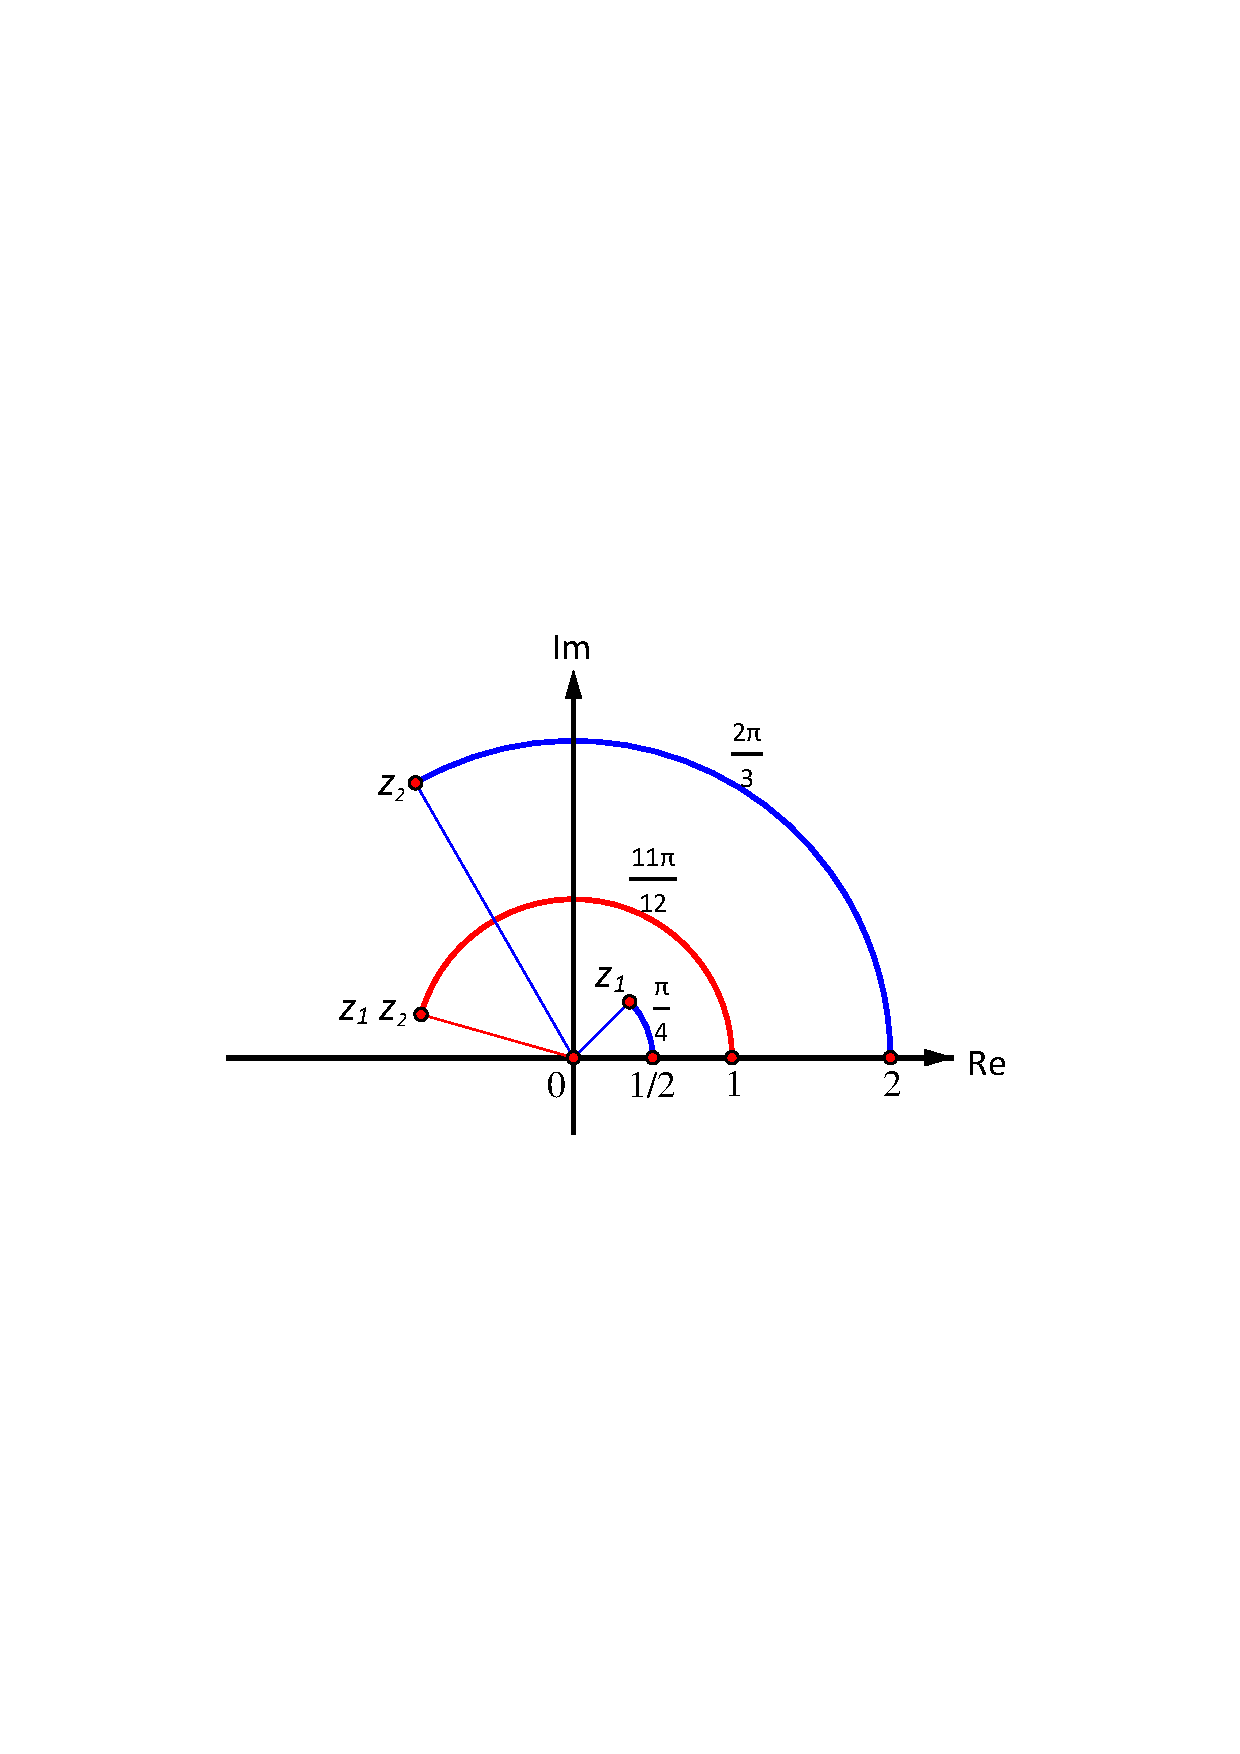
\includegraphics[trim=3cm 10cm 3cm 12cm,width=0.6\textwidth,clip]{Geometer/multiplikation.pdf}\\
Figur 29.10: Multiplikation 
\end{center}
 Vi udregner produktet af $z_1$ og $z_2$ ved hjælp af deres absolutværdier og argumenter:
$$|\,z_1z_2\,|=|\,z_1\,|\,|\,z_2\,|=\frac12\cdot2=1$$
$$\arg(z_1z_2)=\arg(z_1)+\arg(z_2)=\frac{\pi}{4}+\frac{2\pi}{3}=\frac{11\pi}{12}$$
$\,z_1z_2$ er altså det entydigt bestemte tal som har absolutværdien $1$ og argumentet $\frac{11\pi}{12}\,.$
\end{example}
 
\section{Konjugering af komplekse tal}

At konjugere et komplekst tal svarer til at det spejles i realaksen som vist på figur 29.11.
\begin{center}
	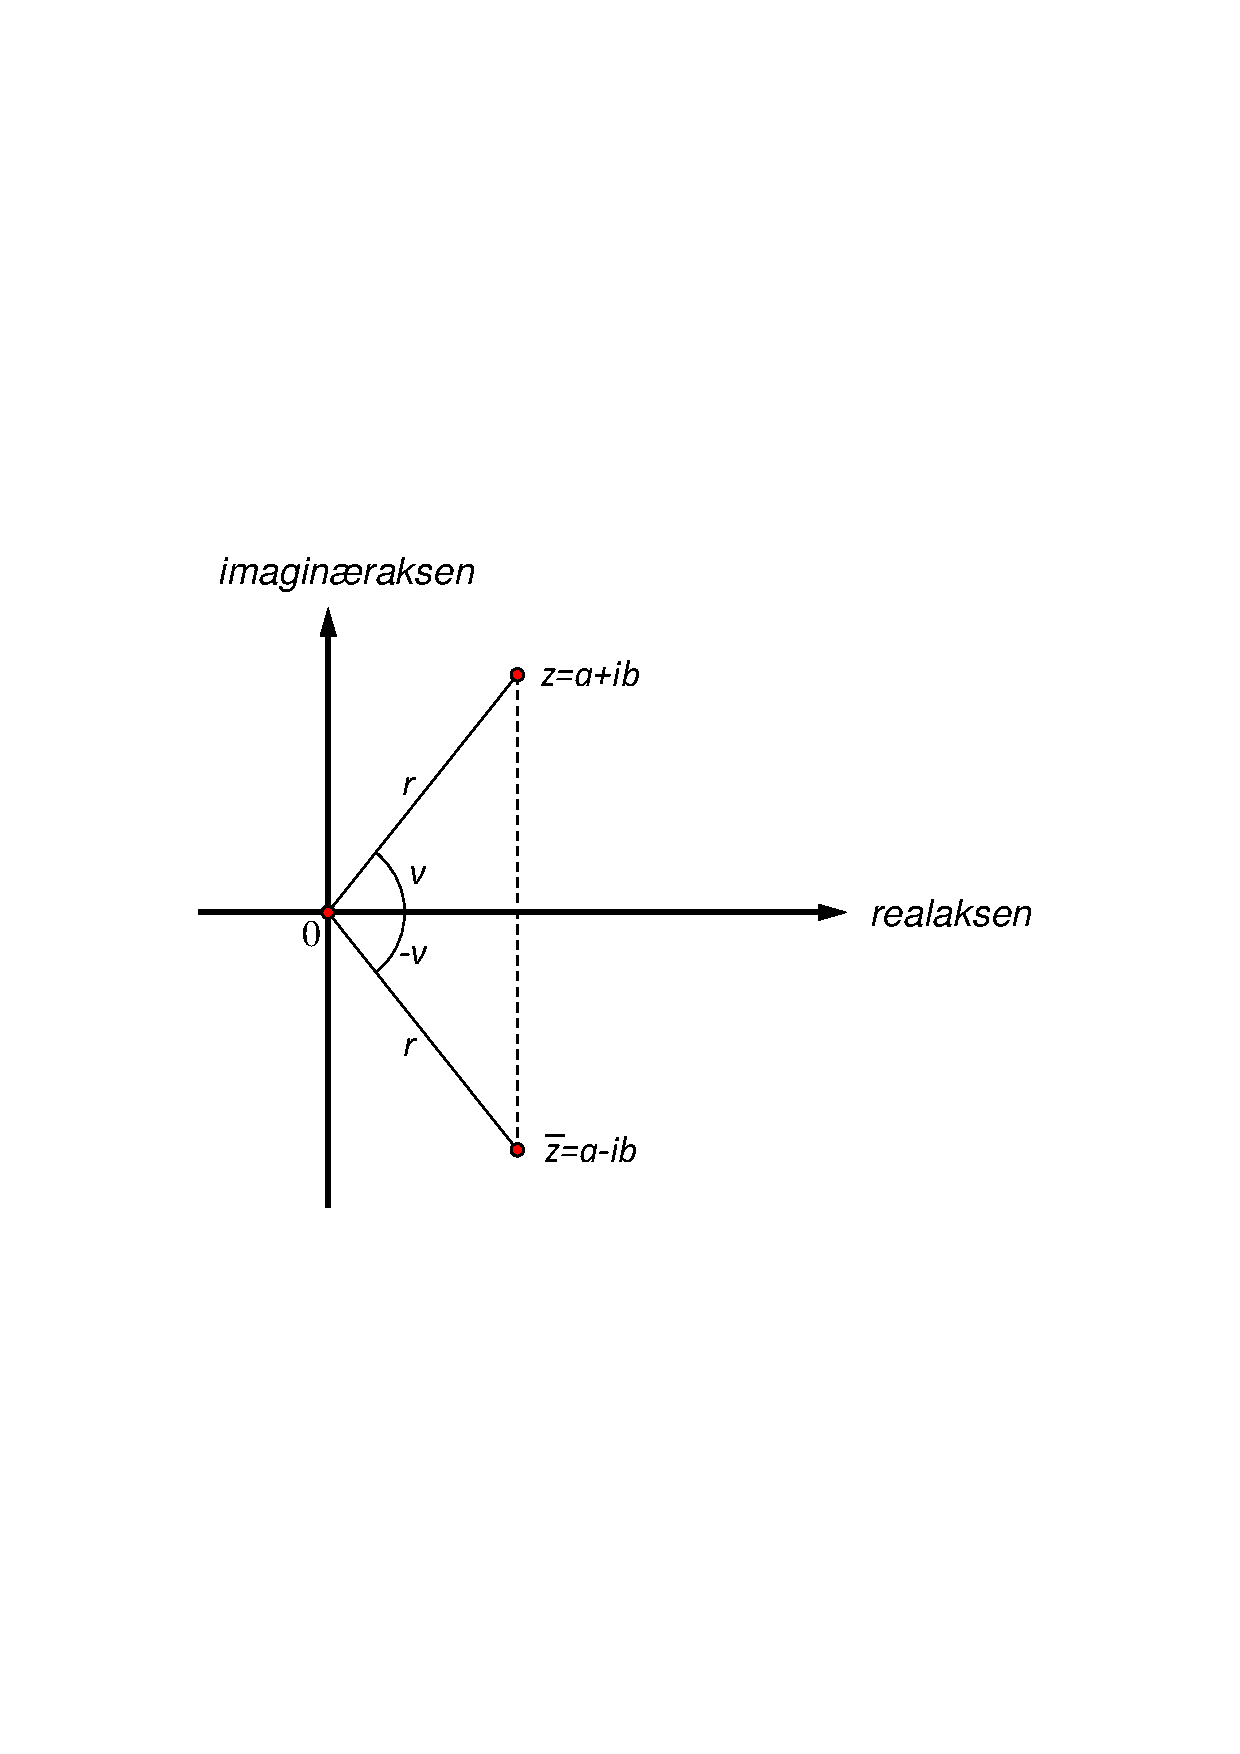
\includegraphics[trim=3cm 9.6cm 3cm 10cm,width=0.6\textwidth,clip]{Geometer/konjugering.pdf}\\
Figur 29.11: Spejling i realaksen 
\end{center}

\begin{definition}
Ved det konjugerede tal til et komplekst tal på rektangulær form $z=a+ib$ forstås tallet $\overline z$ givet ved
\begin{equation}
\overline z=a-ib
\end{equation}
\end{definition}

Det er indlysende at det konjugerede tal til et konjugeret tal er det oprindelige tal selv: 
\begin{equation}
\overline{\overline z}=z\,.
\end{equation}
Det fremgår også klart af definitionen at  konjugerede tal har samme absolutværdi og modsatte argumenter:
\begin{equation}
|\,\overline z\,|=|\,z\,|\,\,\,\mathrm{og}
\,\,\,\arg(\overline z)=-\arg(z)\,.
\end{equation}

Endelig bemærker vi at alle komplekse tal på realaksen er identiske med deres konjugerede tal, og at de er de eneste komplekse tal der opfylder denne egenskab. Vi kan i forlængelse heraf opstille et kriterium for om et givet tal i en en mængde af komplekse tal er reelt:\bs
\begin{theorem}[Realkriteriet]\label{tn29_reeltKriterium}
Lad $A$ være en delmængde af $\mathbb C\,,$ og lad $A_{\mathbb R}$ betegne den delmængde af $A\,$ som består af reelle tal.
Der gælder 
$$A_{\mathbb R}=\left\{z\in A\,|\,\overline z=z\right\}\,.$$
\end{theorem}
\begin{bevis}
Lad $z$ være et vilkårligt tal i $A\,\subseteq \mathbb C$ med rektangulær form $z=a+ib\,.$ Der gælder da 
$$\overline z =z \Leftrightarrow a-ib=a+ib \Leftrightarrow b=0 \Leftrightarrow z\in A_{\mathbb R}\,.$$
\end{bevis}
For konjugering i forbindelse med de fire sædvanlige regnearter gælder der følgende meget simple regneregler\bs
\begin{theorem}[Regneregler for konjugering]\label{tn29-regnKonj}
\begin{enumerate}
\item $\overline{z_1+z_2}=\overline{z_1}+\overline{z_2}$
\item $\overline{z_1-z_2}=\overline{z_1}-\overline{z_2}$
\item $\overline{z_1\cdot z_2}=\overline{z_1}\cdot\overline{z_2}$
%\item $\overline{\frac {z_2}{z_1}}=\frac{\overline {z_2}} {\overline{z_1}}\,\,,\,\,z_1\neq 0\,$
\item $\overline{(z_2/z_1)}=\overline{z_2}/\overline{z_1}\,\,.$
\end{enumerate}

\end{theorem}
\begin{bevis}
Beviset gennemføres ved simpel udregning af formlernes venstreside og højreside
\end{bevis}

\begin{theorem}[Konjugering og absolutværdi]
For et komplekst tal $z$ gælder
\begin{equation}
z\cdot \overline z =|\,z\,|^2
\end{equation}
\end{theorem}
\begin{bevis}
Vi antager at $z=a+ib$ hvor $a$ og $b$ er reelle. Sætningen følger da af
$$
z\cdot \overline z = (a+ib)(a-ib)=a^2+b^2=|\,z\,|^2$$
\end{bevis}

%\begin{aha}
%\end{aha}

\section{Eksponentialfunktion med imaginær variabel}

Den sædvanlige eksponentialfunktion $f(x)=\e^x$ med reel variabel $x$ har som bekendt de karakteristiske egenskaber 
\begin{equation}
\e^0=1\quad \mathrm{og} \quad\,\e^{x_1+x_2}=\e^{x_1}\cdot\e^{x_2}\,.
\end{equation}
Ved gentagen brug af den sidste får vi desuden  egenskaben 
\begin{equation}
(\e^{x})^n=\e^{nx}\quad ,\,n\in \mathbb N\,.
\end{equation}

I dette afsnit vil vi indføre en  eksponentialfunktion med \textit{imaginær variabel}, som senere i denne eNote udvides til en kompleks eksponentialfunktion $f(z)=\e^z$ for ethvert $z\in \mathbb C\,$. Vi vil kræve at $f(z)$ stemmer overens med den reelle eksponentialfunktion når $z\in \mathbb R\,,$ og at $f(z)$ besidder de samme karakteristiske egenskaber som den reelle. Men her starter vi med specialtilfældet at variablen er rent imaginær.

\begin{definition}\label{tn29_eiy}
For ethvert $v\in \mathbb R\,$ defineres funktionen  $\e^{iv}$ ved
\begin{equation}
\e^{iv}=\cos(v)+i\sin(v)\,.
\end{equation}
\begin{center}
	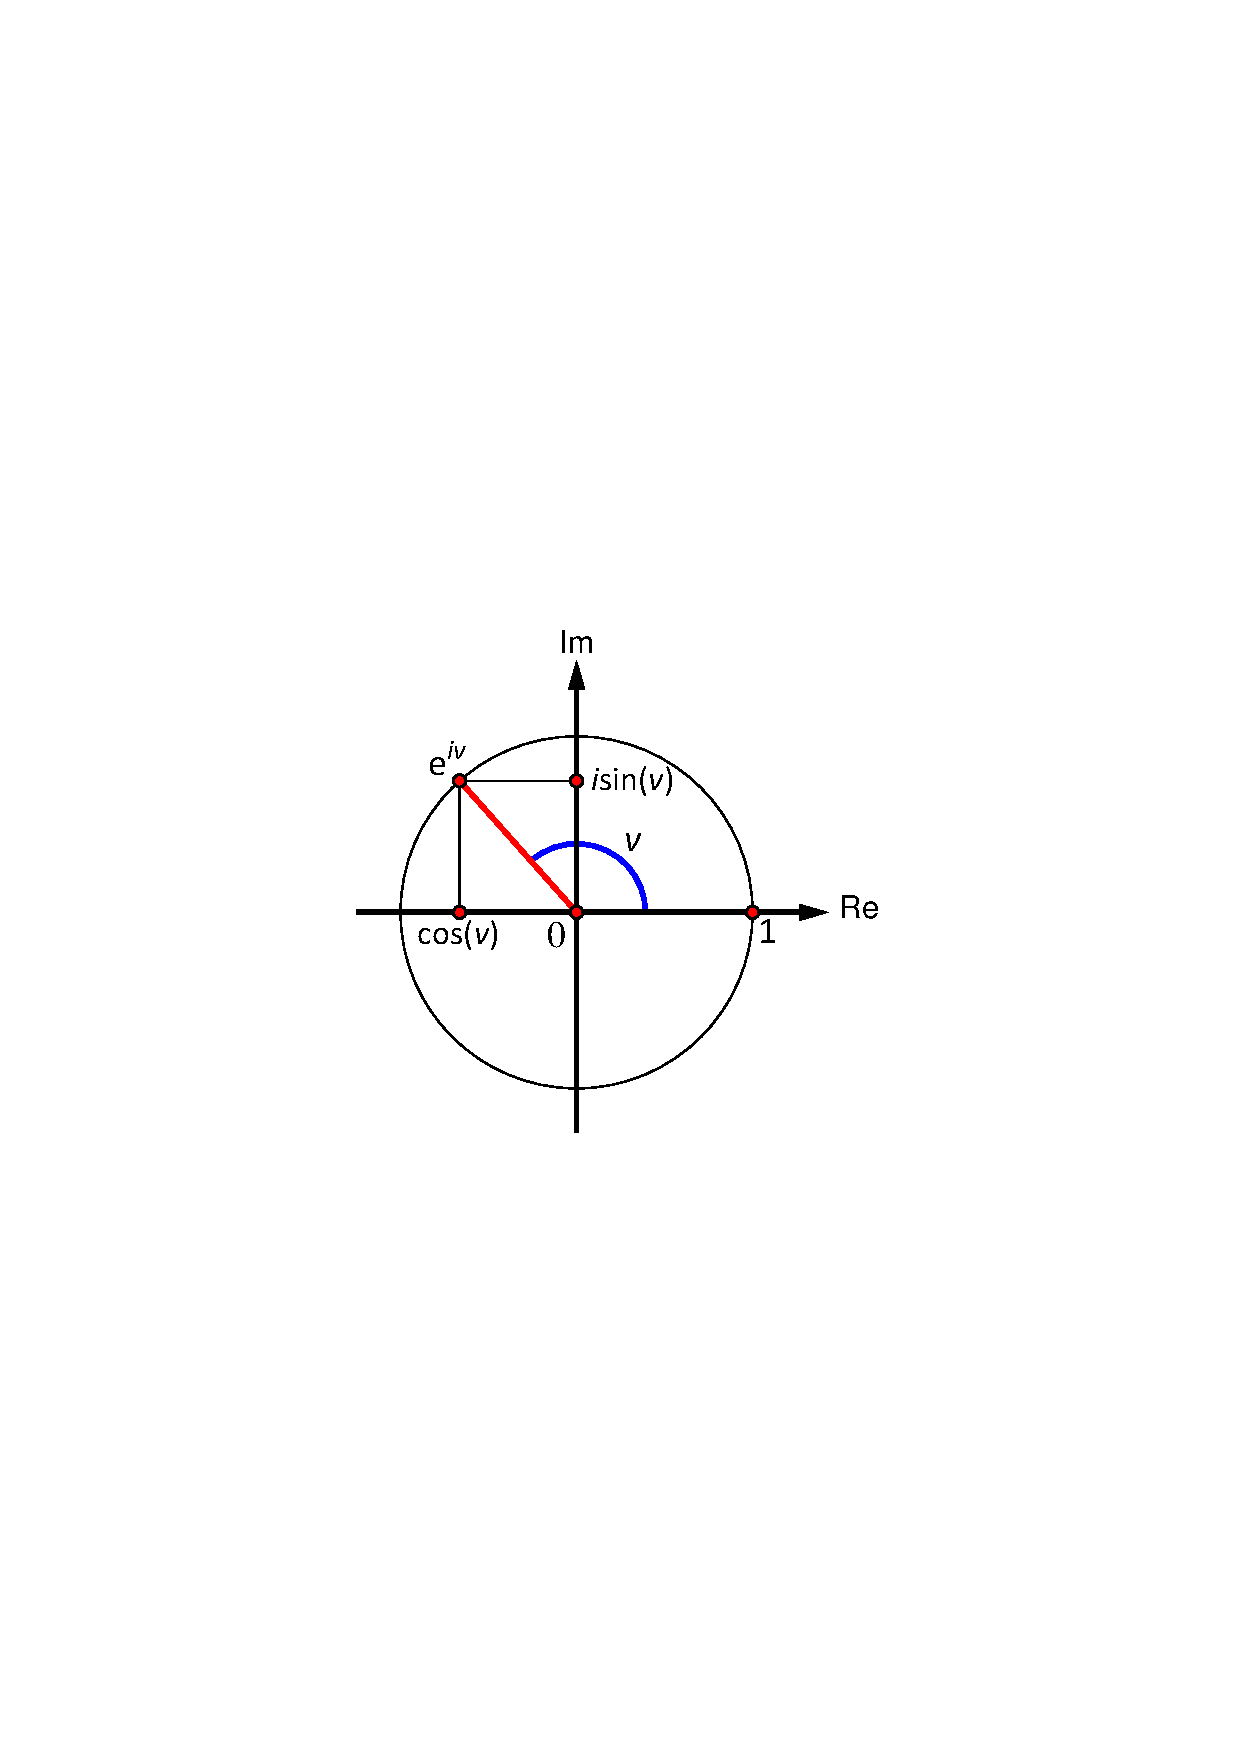
\includegraphics[trim=3cm 10.7cm 3cm 10.7cm,width=0.6\textwidth,clip]{Geometer/exp_iv.pdf}\\
Figur 29.12: Enhedscirklen i komplekse talplan 
\end{center}
\end{definition}

\begin{aha}
Bemærk at tallet $\e^{iv}$ for ethvert $v$ ligger på enhedscirklen i den komplekse talplan med centrum i $0\,$. Heraf følger:
\begin{equation}
|\,\e^{iv}\,|=1\,.
\end{equation}
Bemærk endvidere at argumentet for $\e^{iv}$ straks aflæses i eksponenten således:
\begin{equation}
\arg(\e^{iv})=v\,.
\end{equation}
\end{aha}
Vi viser nu at den i definition \ref{tn29_eiy} indførte funktion $\e^{iv}$ har egenskaber der svarer til den reelle eksponentialfunktion.\bs 
\begin{theorem}[Regneregler for $\e^{iv}$]\label{tn29_Th_eiy}
For funktionen $\e^{iv}\,\,,\,v\in \reel$ gælder
\begin{enumerate}
\item
$\e^{0i}=1$
\item
$\e^{iv_1+iv_2}=\e^{i(v_1+v_2)}=\e^{iv_1}\e^{iv_2}$
\item
$(\e^{iv})^n=\e^{inv}\,\,,\,n\in\mathbb N$
\end{enumerate}
\end{theorem}
\begin{bevis}
\begin{enumerate}
\item
Der gælder oplagt $\e^{i0}=\cos(0)=1\,.$
\item
Lad $v_1$ og $v_2$ være to reelle tal. Fra (\ref{tn29_RegnAbs1}) fås $$|\,\e^{iv_1}\e^{iv_2}\,|=|\,\e^{iv_1}\,|\,|\,\e^{iv_2}\,|=1\,.$$
Fra (\ref{tn29_RegnArg1}) fås $$\arg(\e^{iv_1}\e^{iv_2})=\arg(\e^{iv_1})+\arg(\e^{iv_2})=v_1+v_2\,.$$
Nu indsætter vi den fundne absolutværdi og argument for $\e^{iv_1}\e^{iv_2}\,$ i dette tals eksponentielle form: 
$$\e^{iv_1}\e^{iv_2}=\e^{i(v_1+v_2)}=\e^{iv_1+iv_2}\,.$$
\item
På tilsvarende vis fås fra (\ref{tn29_RegnAbs3}) og (\ref{tn29_RegnArg3}) at 
\begin{equation}
(\e^{iv})^n=\e^{inv}\,.
\end{equation}
\end{enumerate}
\end{bevis}

Vi kan herefter indføre en i mange sammenhænge bekvem og meget benyttet skrivemåde for komplekse tal.

\begin{theorem}[Eksponentiel form]
Ethvert komplekst tal $z$ kan skrives på formen
\begin{equation}\label{tn29_ekspForm1}
z=r\e^{iv}\,,
\end{equation}
hvor $r=|\,z\,|$ og $v=\arg(z)\,$. Skrivemåden kaldes tallets \textit{eksponentielle form}.
\end{theorem}
\begin{bevis}
Vi finder først absolutværdi af $r\e^{iv}\,$:
$$|\,r\e^{iv}\,|=|\,r\,|\,|\,\e^{iv}\,|=r\,.$$
Dernæst et argument for $r\e^{iv}\,$:
$$\arg(r\e^{iv})=\arg(r)+\arg(\e^{iv})=0+v=v\,.$$ 
Hermed er det vist at $z$ og $r\e^{iv}$ har samme absolutværdi og samme argument, og derfor er identiske.
\end{bevis}

Når komplekse tal angives på eksponentiel form, foregår multiplikation, division og potensopløftning uden videre efter sædvanlige elementære regneregler og potensregler kendt fra reelle tal. Vi giver nu et eksempel på dette i forbindelse med multiplikation, sammenlign med eksempel \ref{PolarMult}.

\begin{example}[Multiplikation på eksponentiel form]
To komplekse tal er givet på eksponentiel form:
$$z_1=\frac 12\,\e^{\frac{\pi}{4} i}\,\,\,\mathrm{og}\,\,\,
z_2=2\,\e^{\frac{3\pi}{2} i}\,.$$
Produktet af tallene fås på eksponentiel form ved
$$z_1z_2=\big(\frac 12\,\e^{\frac{\pi}{4}i}\big)\big(2\,\e^{\frac{3\pi}{2}i}\big)=
(\frac 12\cdot 2)\e^{\frac{\pi}{4}i+\frac{3\pi}{2}i}=
1\e^{i(\frac{\pi}{4}+\frac{3\pi}{2})}=
\e^{\frac{7\pi}{4}\,i}\,.
$$
\end{example}
I det følgende vil vi vise hvordan såkaldte \textit{binome ligninger} kan løses ved hjælp af eksponentiel form. En binom ligning er en \textit{toleddet} polynomiumsligning med formen
\begin{equation}
z^n=w
\end{equation}
hvor $w\in \mathbb C\,$ og $n\in\mathbb N\,$.\bs

Vi viser først et eksempel på løsning af en binom ligning ved hjælp af eksponentiel form og opstiller derefter den generelle metode.

\begin{example}[Binom ligning på eksponentiel form]\label{tn29_binom}
Find samtlige løsninger på den binome ligning
\begin{equation}\label{tn29_binom1}
z^4=-8+8\sqrt 3 i\,.
\end{equation}
Løsning:\\
Ideen er at vi skriver såvel $z$ som højresiden på eksponentiel form.\bs 
Hvis $z$ har den eksponentielle form $z=s\e^{iu}\,$, kan ligningens venstreside udregnes ved 
\begin{equation}\label{tn29_binom2}
z^4=(s\e^{iu})^4=s^4\,(e^{iu})^4=s^4\,e^{i4u}
\end{equation}
Højresidens absolutværdi $r$ findes ved
$$r=|\,-8+8\sqrt 3\,|=\sqrt{(-8)^2+(8\sqrt 3)^2}=16\,.$$
Højresidens argument $v$ opfylder:
$$\cos(v)=\frac{-8}{16}=-\frac{1}{2}\,\,\,\mathrm{og}\,\,\,
\sin(v)=\frac{8\sqrt 3} {16}=\frac{\sqrt 3}{2}\,.$$
Ved hjælp af de to ligninger kan højresidens hovedargument fastlægges til 
$$v=\mathrm{Arg}(-8+8\sqrt 3)=\frac {2\pi}3\,,$$
og dermed den eksponentielle form
\begin{equation}\label{tn29_binom3}
r\e^{iv}\,=16\e^{\frac {2\pi}3\,i}\,.
\end{equation}
Vi indsætter nu (\ref{tn29_binom2}) og (\ref{tn29_binom3}) i (\ref{tn29_binom1})
$$
s^4\,e^{i4u}=16\e^{\frac {2\pi}3\,i}\,.
$$
Da ventresidens absolutværdi skal være lig højresidens får vi
$$
s^4=16\,\,\Leftrightarrow\,\, s=\sqrt[4]{16}=2.
$$

Venstresidens argument $4u$ og højresidens argument $\frac {2\pi}3$ skal være ens på nær et multiplum af $2\pi\,$. Heraf fås
$$4u=\frac {2\pi}3+p2\pi\,\,
\Leftrightarrow\,\, u =\frac {\pi}6 +p\frac {\pi}2 \,\,,\,\,p\in \mathbb Z\,.
$$
Disse uendeligt mange argumenter svarer vel at mærke kun til \textit{fire} halvlinjer ud fra $0\,$, bestemt ved de argumenter der fås ved $p=0,p=1,p=2$ og $p=3\,$. For alle andre værdier af $p$ vil den tilsvarende halvlinje være identisk med en af de fire nævnte. For eksempel vil halvlinjen for $p=4$ være givet ved argumentet
$$u=\frac {\pi}6 +4\,\frac{\pi}2=\frac {\pi}6+2\pi\,,$$
det vil sige samme halvlinje som svarer til $p=0\,$, da forskellen på argumenterne er $2\pi\,$.\bs
Den givne ligning (\ref{tn29_binom1}) har derfor netop fire løsninger, som ligger på de nævnte fire halvlinjer i afstanden $s=2$ fra $0\,$. Angivet på  eksponentiel form:
$$z=2\,\e^{i(\frac {\pi}6 +p\frac {\pi}2 )}\,\,,\,\,p=0\,,\,1\,,\,2\,,\,3\,.$$
Eller omregnet hver for sig til rektangulær form ved brug af definition \ref{tn29_eiy}
$$z_0=\sqrt 3+i\,,\,z_1=-1+i\sqrt 3\,,\,z_2=-\sqrt 3-i\,,\,z_3=1-i\sqrt 3\,.$$
\end{example}

Alle løsningerne for en binom ligning ligger på en cirkel med centrum i $0$ og radius lig med højresidens absolutværdi.  Forbindelseslinjerne mellem Origo og løsningerne deler cirklen i lige store vinkler som det eksemplificeres på figur 29.13. 

\begin{center}
	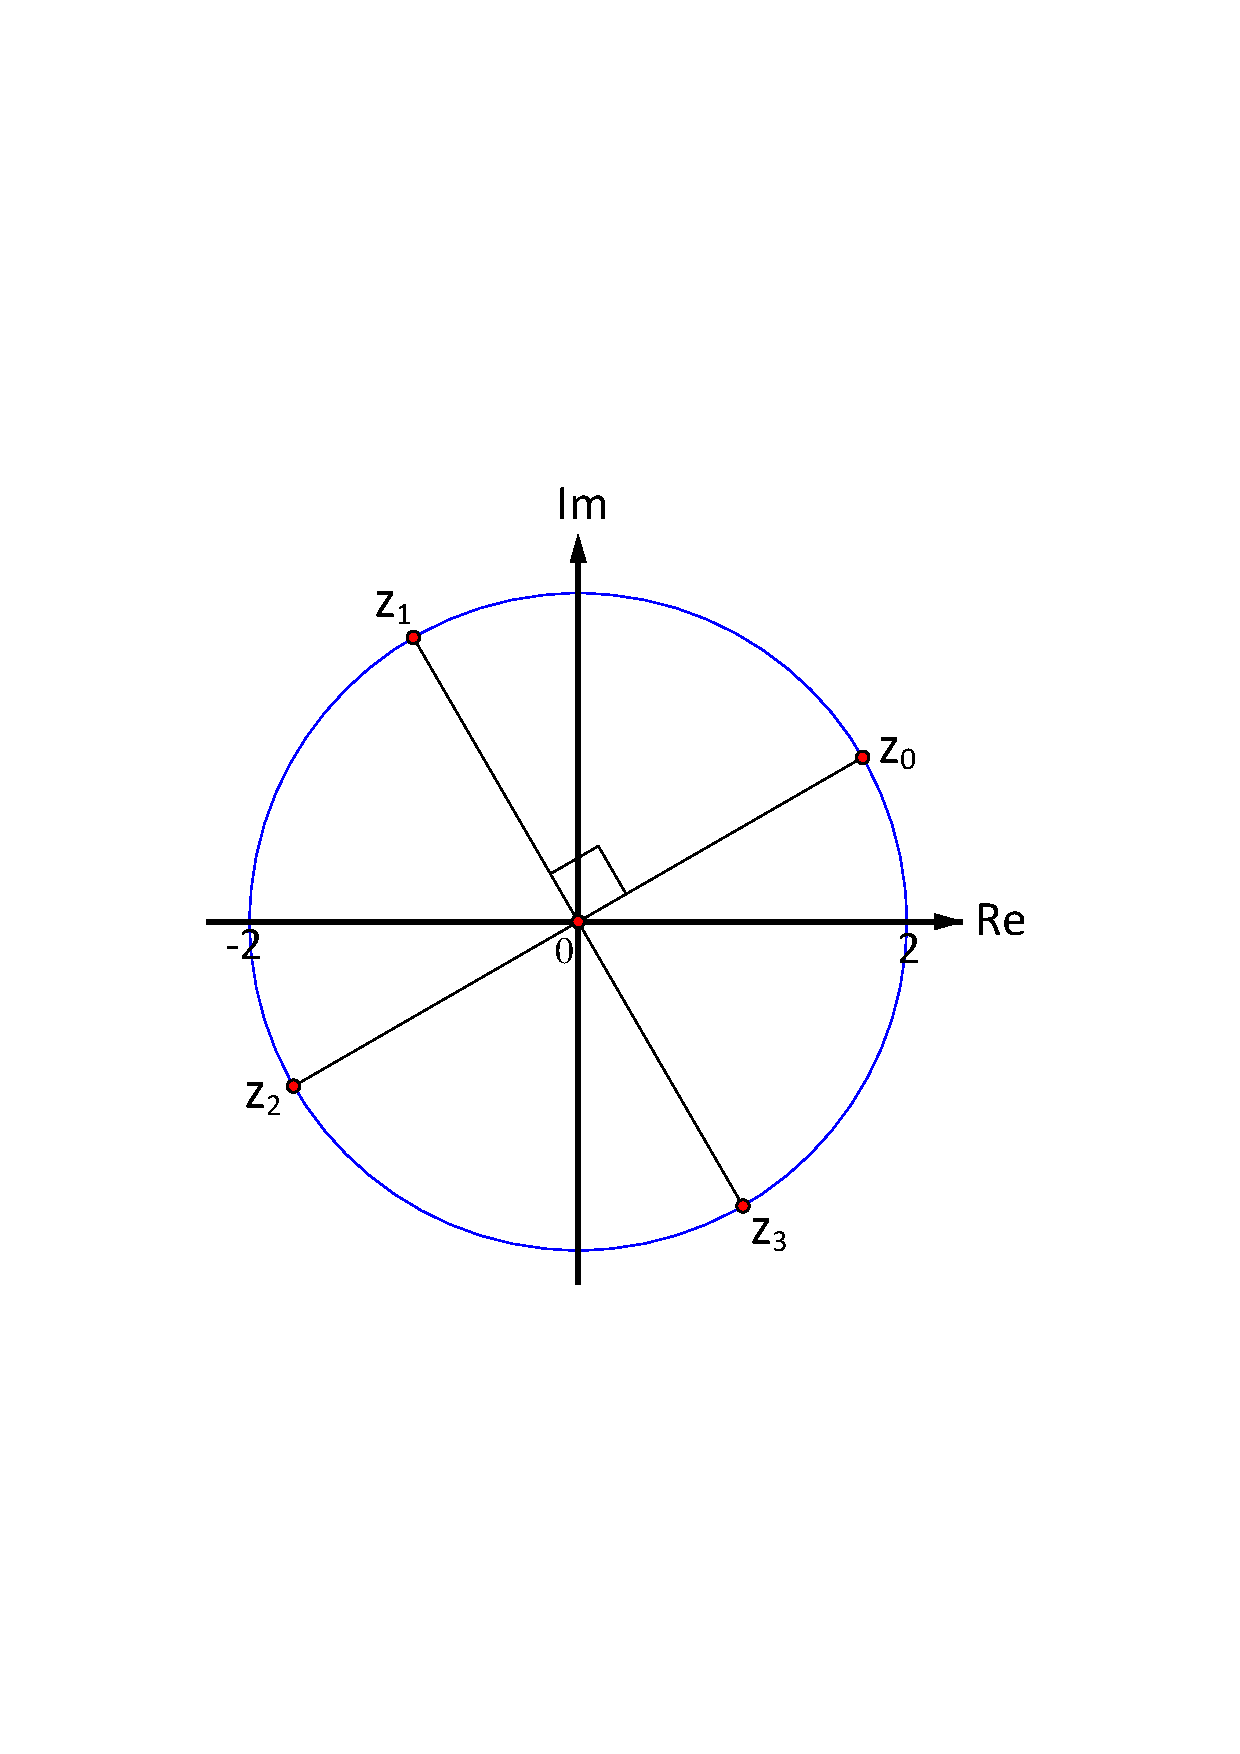
\includegraphics[trim=3cm 7.8cm 3cm 9.2cm,width=0.4\textwidth,clip]{Geometer/4lsn.pdf}\\
Figur 29.13: Løsningerne fra eksempel \ref{tn29_binom}
\end{center}


Fremgangsmåden i eksempel \ref{tn29_binom} generaliserer vi i den følgende sætning. Sætningen bevises i eNote 30 om polynomier.

\begin{theorem}[Binom ligning løst vha. eksponentiel form]
Givet et komplekst tal $w\,$, som ikke er $0\,$, og som har den eksponentielle form
$$w=r\e^{iv}\,.$$
Den binome ligning
\begin{equation}
z^n=w=r\e^{iv}\,\,,\,n\in \mathbb N
\end{equation}
har $n$ løsninger som kan findes ved formlen
\begin{equation}
z=\sqrt[n]{r}\,\,\e^{i(\frac vn+p\frac{2\pi}n)}\,\,\,\mathrm{hvor} \,\,\,
p=0\,,\,1\,,...\,,\,n-1\,.
\end{equation}
\end{theorem}
\section{Den komplekse eksponentialfunktion}

Som tidligere nævnt i denne eNote er det muligt at udvide  definitionsmængden for den velkendte reelle eksponentialfunktion $\e^x$ fra de reelle tal til de komplekse tal, således at den udvidede komplekse eksponentialfunktion på realaksen svarer overens med den reelle. Og således at de karakteristiske egenskaber for den reelle eksponentialfunktion overføres til den komplekse. 

\begin{definition}[Kompleks eksponentialfunktion]\label{tn29_ez}
For et hvert komplekst tal $z$ med rektangulær form $z=x+iy$ defineres den komplekse eksponentialfunktion $\e^z$ ved
\begin{equation}\label{tn29_ez1}
\e^z=\e^{x+iy}=\e^x\e^{iy}=\e^x\big(\cos(y)+i\sin(y)\,\big)\,.
\end{equation}
\end{definition}

\begin{aha}
Bemærk at hvis $z$ i (\ref{tn29_ez1}) er reel, det vil sige hvis $y=0\,$, så er (\ref{tn29_ez1}) den sædvanlige reelle eksponentialfunktion $\e^x\,.$\bs
Bemærk at hvis $x=0$ i (\ref{tn29_ez1}), så er (\ref{tn29_ez1}) den i definition \ref{tn29_eiy} indførte eksponentialfunktion for ren imaginær variabel.
\end{aha}

Vi betragter nu det komplekse tal $\e^z$ hvor $z$ er et vilkårligt komplekst tal med rektangulær form $z=x+iy$ hvor ikke både $x$ og $y$ er lig med $0$. Vi har umiddelbart fra definition \ref{tn29_ez} den \textit{eksponentielle form} af $\e^z\,$
$$
\e^z=\e^x\e^{iy}\,,
$$
der viser at
$$
|\,\e^z\,|=\e^x\,\,\,\mathrm{og} \,\,\,\arg{\e^z}=y\,.
$$ 
Dette giver $\e^z$ en bemærkelsesværdig placering i den komplekse talplan som vist på figur 29.14.

\begin{center}
	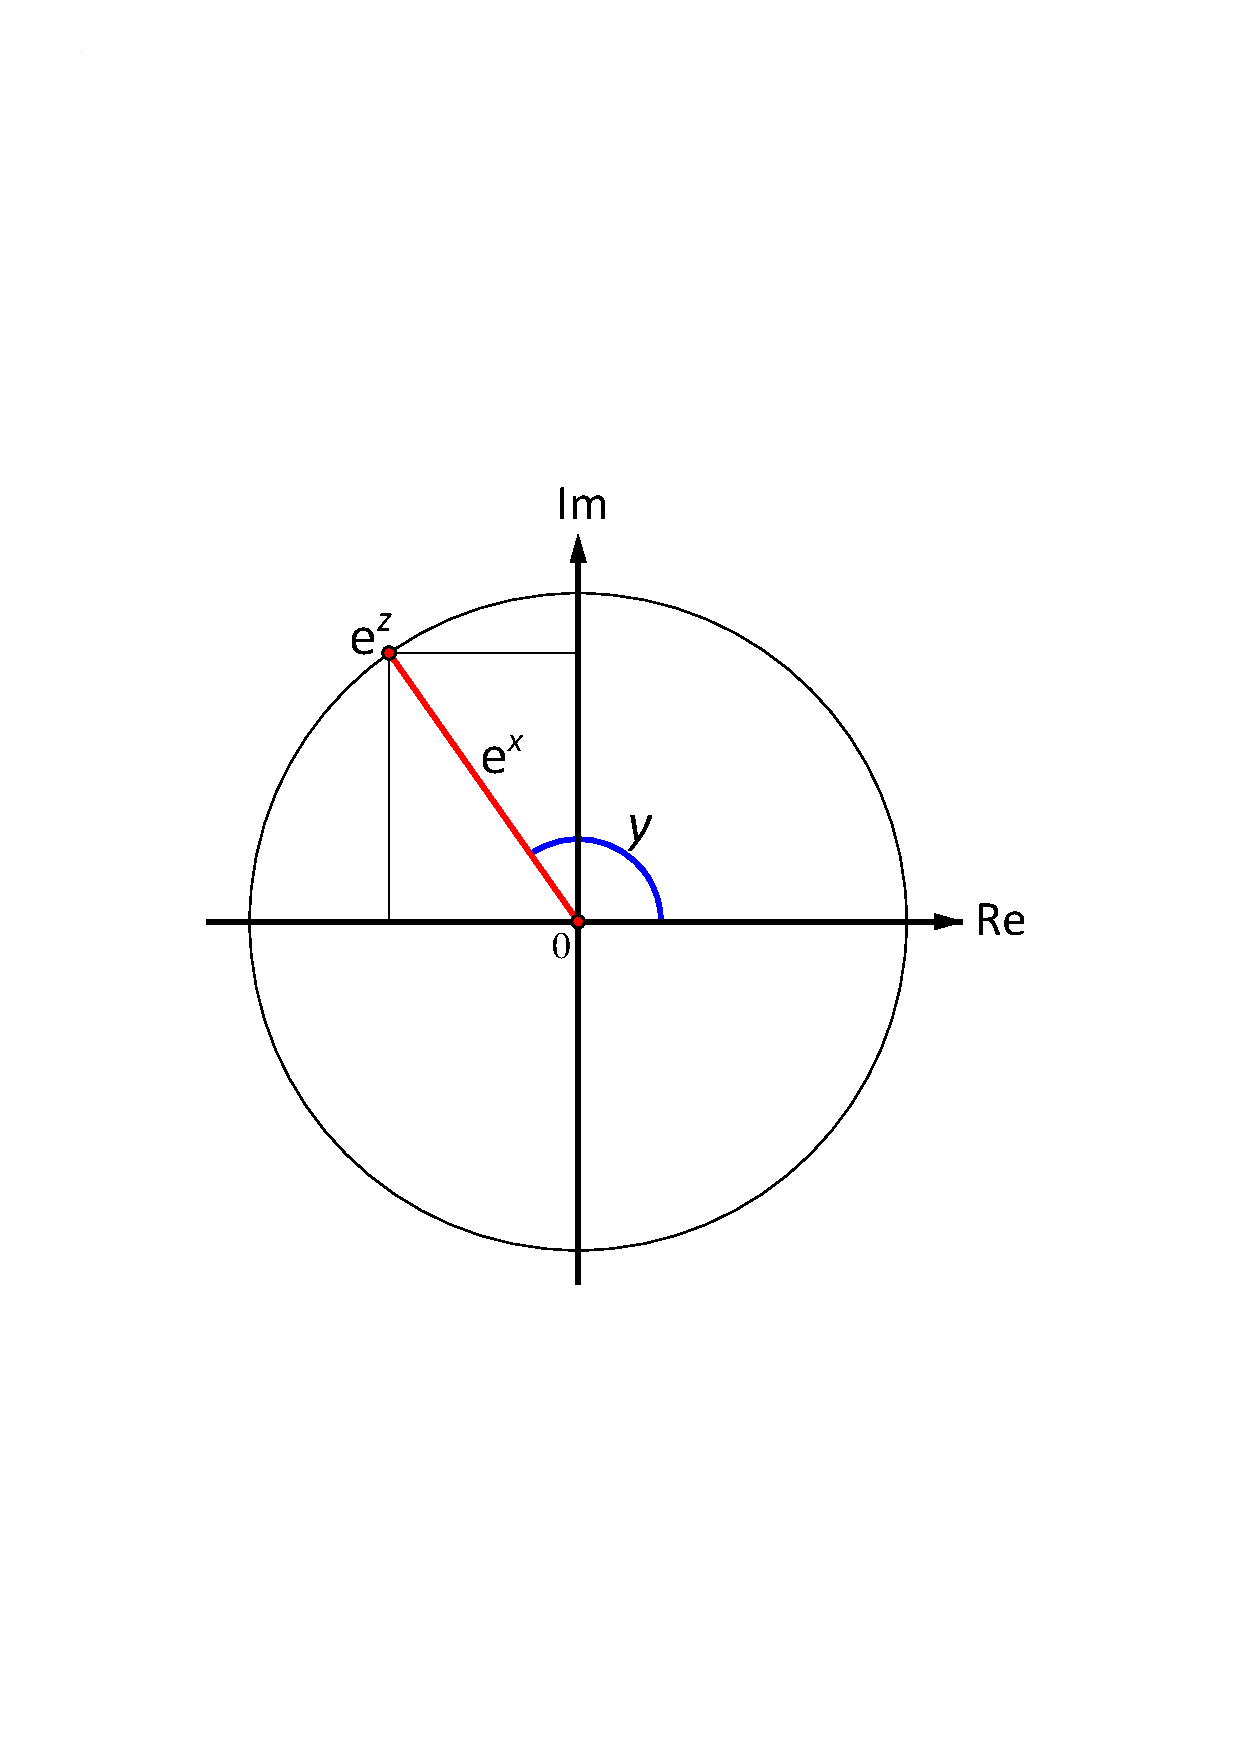
\includegraphics[trim=3cm 7.5cm 3cm 9cm,width=0.4\textwidth,clip]{Geometer/eksponentielForm2.pdf}\\
Figur 29.14: Geometrisk fortolkning af $\e^z$
\end{center}

\begin{example}[Eksponentiel ligning]\label{exEkspLign}
Bestem samtlige løsninger for ligningen
\begin{equation}\label{exEkspLign1}
\e^z=-\sqrt 3+i\,.
\end{equation}
Løsning:\\
Vi skriver først $z$ på rektangulær form: $z=x+iy\,$.\\ 
I eksempel \ref{tn29_exOmform} har vi fundet at højresiden i \ref{exEkspLign1} har absolutværdien $r=2$ og hovedargumentet $v=\frac{5\pi}6\,$. Da venstresiden og højresiden skal have samme absolutværdi og samme argument på nær et vilkårligt multiplum af $2\pi\,$ fås
$$
|\,\e^z\,|=\e^x=r=2\,\,\Leftrightarrow\,\,x=\ln(2)\,,$$
$$\arg(z)=y=v+p2\pi=\frac{5\pi}6 + p2\pi\,\,,\,p\in \mathbb Z\,.$$
Samtlige løsninger for \ref{exEkspLign1} er dermed
$$z=x+iy=\ln(2)+i(\frac{5\pi}6 + p2\pi)\,\,,\,p\in \mathbb Z\,.$$
 
\end{example}

For de reelle trigonometriske funktioner $\cos(x)$ og $\sin(x)$ vides at der for ethvert helt tal $p$ gælder $\cos(x+p2\pi)=\cos(x)$ og $\sin(x+p2\pi)=\sin(x)\,$. Hvis man forskyder grafen for $\cos(x)$ eller $\sin(x)$ med et vilkårligt multiplum af $2\pi\,$, vil den derfor gå over i sig selv. Funktionerne kaldes derfor \textit{periodiske} med \textit{perioden} $2\pi\,$.\bs
Et lignende fænomen kan ses i eksempel \ref{exEkspLign} hvor den givne eksponentielle lig\-ning har uendeligt mange løsninger der kun adskiller sig fra hinanden ved forskellige multipla af $2\pi i\,$. Det skyldes at den komplekse eksponentialfunktion har den ima\-ginære periode $2\pi i\,$! Og dette hænger i høj grad sammen med periodiciteten af de trigonometriske funktioner.

\begin{theorem}[Periodicitet af $\e^z$]
For ethvert komplekst tal $z$ og ethvert helt tal $p$ gælder
\begin{equation}
\e^{z+p2\pi i}=\e^z\,.
\end{equation}
\end{theorem}
\begin{bevis}
Antag at $z$ har rektangulær form $z=x+iy\,$ og $p\in \mathbb Z\,.$\bs
Der gælder
$$
\e^{z+p2\pi i}
=\e^{x+i(y+p2\pi)}
=\e^x\big(\cos(y+p2\pi)+i\sin(y+p2\pi)\,\big)$$
$$=\e^x\big(\cos(y)+i\sin(y)\,\big)
=\e^z\,.$$
Hermed er sætningen vist.
\end{bevis}
Vi viser nu at $\e^z$ faktisk har den karakteristiske ``eksponentielle'' egenskab kendt fra den reelle eksponentialfunktion og som i \ref{tn29_Th_eiy} blev udvidet til eksponentialfunktionen med imaginær variabel.\bs 
\begin{theorem}[Regneregel for $\e^z$]\label{tn29_Th_ez}
For vilkårlige komplekse tal $z_1$ og $z_2$ opfylder den komplekse eksponentialfunktion
\begin{equation}
\e^{z_1+z_2}=\e^{z_1}\cdot\e^{z_2}\,.
\end{equation}
\end{theorem}
\begin{bevis}
Med i næste opdatering af eNoten.
\end{bevis}

\section{Komplekse funktioner af en reel variabel}

Lad $c$ være et vilkårligt komplekst tal. Vi vil til ethvert reelt tal $t$ knytte det komplekse tal
\begin{equation}\label{tn29_komplFunk}
f(t)=\e^{ct}\,.
\end{equation}
Denne funktion er et eksempel på de såkaldte \textit{komplekse funktioner af en reel variabel}, som vi indfører generelt i det følgende. Derefter  fokuseres specielt på typen (\ref{tn29_komplFunk}) der har vid udbredelse i såvel teoretisk som anvendt matematik. \bs

\begin{definition}[Kompleks funktion af reel variabel]
Ved en \textit{kompleks funktion} $f:\reel\longrightarrow \mathbb C$
af en reel variabel $t$ forstås en funktion af typen
\begin{equation}
f(t)=g(t)+i\cdot h(t)
\end{equation}
hvor $g(t)$ og $h(t)$ er reelle funktioner af den reelle variable $t$.\bs
$f(t)$ kaldes \textit{differentiabel} hvis $g(t)$ og $h(t)$ begge er differentiable.\\
Differentialkvotienten af $f(t)$ defineres ved
\begin{equation}\label{tn29_defDiff2}
f'(t)=g'(t)+i\cdot h'(t)\,.
\end{equation}
\end{definition}

\begin{example}[Kompleks funktion af reel variabel]
Ved udtrykket
$$f(t)=t+it^2\,\,,\,t\in\reel$$
er der defineret en kompleks funktion af en reel variabel. Den har differentialkvotienten
$$f'(t)=1+i(2t)\,.$$
\end{example}

\begin{example}[Kompleks funktion af reel variabel]
Den i definition \ref{tn29_eiy} indførte funktion 
$$g(t)=\e^{it}=\cos(t)+i\sin(t)\,\,,\,t\in\reel\,$$
er en kompleks funktion af en reel variabel. Den  har differentialkvotienten
$$g'(t)=-\sin(t)+i\cos(t)\,.$$
\end{example}

De sædvanlige regneregler for differentiable funktioner udvides nemt til regneregler for differentialble komplekse funktioner af reel variabel. I den følgende sætning betragter vi de såkaldte \textit{lineære} egenskaber ved differentiation.

\begin{theorem}[Regneregler for differentialkvotient]\label{tn29_regnDiff}
Lad $f_1(t)$ og $f_2(t)$ være komplekse funktioner af den reelle variable $t\,,$ og lad $c$ være et vilkårligt komplekst tal. Der gælder da\bs
1. Den komplekse funktion $f_1(t)+f_2(t)$ er differentiabel med differentialkvotienten 
\begin{equation}
\big (\,f_1(t)+f_2(t)\,)'=f_1'(t)+f_2'(t)\,.
\end{equation}
2. Den komplekse funktion $c\cdot f_1(t)$ er differentiabel med differentialkvotienten 
\begin{equation}
\big (\,c\cdot f_1(t)\,\big)'=c\cdot f_1'(t)
\end{equation}
\end{theorem}

\begin{bevis}
Lad $f_1(t)=g_1(t)+i\,h_1(t)$ og $f_2(t)=g_2(t)+i\,h_2(t)$ hvor $g_1(t),\,h_1(t),\,g_1(t)$ og $g_2(t)$ er differentiable reelle funktioner. Lad endvidere $c=a+ib$ være et vilkårligt komplekst tal på rektangulær form.\bs
Sætningens første del:\\
$
\begin{aligned}
f_1(t)+f_2(t)&=\left(g_1(t)+i\,h_1(t)\right)+\left(g_2(t)+i\,h_2(t)\right)\\
&=\left(g_1(t)+g_2(t)\right)+i\left(h_1(t)+h_2(t)\right)\,.
\end{aligned}
$\bs
Vi får da fra definition (\ref{tn29_defDiff2}) og brug af regneregler for differentialkvotienter af reelle funktioner:\bs
$
\begin{aligned}
\left(f_1(t)+f_2(t)\right)'&=\left(g_1(t)+g_2(t)\right)'+i\left(h_1(t)+h_2(t)\right)'\\
&=\left(g_1'(t)+g_2'(t)\right)+i\left(h_1'(t)+h_2'(t)\right)\\
&=\left(g_1'(t)+i\,h_1'(t)\right)+i\left(g_2'(t)+i\,h_2'(t)\right)\\
&=f_1'(t)+f_2'(t)\,.
\end{aligned}
$\bs
%Hermed er sætningens første del bevist\bs
Sætningens anden del:\\
$
\begin{aligned}
c\cdot f_1(t)&=(a+ib)\cdot\left(g_1(t)+i\,h_1(t)\right)\\
&=\left(a\,g_1(t)-b\,h_1(t)\right)+i\left(a\,h_1(t)+b\,g_1(t)\right)
\end{aligned}
$\bs
Vi får fra definition (\ref{tn29_defDiff2}) og brug af regneregler for differentialkvotienter af reelle funktioner:\bs
$
\begin{aligned}
\left(c\cdot f_1(t)\right)'&=\left(a\,g_1(t)-b\,h_1(t)\right)'+i\left(a\,h_1(t)+b\,g_1(t)\right)'\\
&=\left(a\,g_1'(t)-b\,h_1'(t)\right)+i\left(a\,h_1'(t)+b\,g_1'(t)\right)\\
&=(a+ib)\left(g_1'(t)+h_1'(t)\right)\\
&=c\cdot f_1'(t)\,.
\end{aligned}
$\bs
Hermed er sætningen bevist.
\end{bevis}

%\begin{definition}[Stamfunktion]
%Ved en stamfunktion til en kompleks funktion $f(t)\,\,,\,t\in \reel\,$ forstås en kompleks funktion $F(t)\,\,,\,t\in \reel\,$ der opfylder
%\begin{equation}
%F'(t)=f(t)\,.
%\end{equation}
%\end{definition}

%\begin{theorem}
%Lad $$
%\end{theorem}

Vi vender nu tilbage til funktioner af typen (\ref{tn29_komplFunk}). Først giver vi et nyttigt resultat om deres konjugering:

\begin{theorem}\label{tn29-konj_ect}
For et vilkårligt komplekst tal $c$ og ethvert reelt tal $t$ gælder
\begin{equation}
\overline{\e^{ct}}=\e^{\overline c \,t}\,.
\end{equation}
\end{theorem}

\begin{bevis}
Lad $c=a+ib\,$ være den rektangulære form af $c\,.$ Vi får da ved brug af definition \ref{tn29_ez} og regneregler \ref{tn29-regnKonj} for konjugering:\bs
$
\begin{aligned}
\overline{\e^{ct}}&=\overline{\e^{at+ibt}}\\
&=\overline{e^{at}\left(\cos(bt)+i\sin(bt)\right)}\\
&=\overline{e^{at}}\,\,\overline{\left(\cos(bt)+i\sin(bt)\right)}\\
&=e^{at}\left(\cos(bt)-i\sin(bt)\right)\\
&=e^{at}\left(\cos(-bt)+i\sin(-bt)\right)\\
&=e^{at-ibt}\\
&=e^{\overline{c}t}\,.
\end{aligned}
$\bs

Hermed er sætningen bevist.
\end{bevis}


For sædvanlige reelle eksponentialfunktioner af typen 
$$f(x)=\e^{kx}\,\,,\,k\in\reel\,$$
gælder der som bekendt
\begin{equation}\label{tn29_diffekx}
f'(x)=kf(x)=k\e^{kx}\,.
\end{equation}
Vi slutter eNoten af med at vise at den komplekse eksponentialfunktion opfylder en differentiationsregel der helt svarer til \ref{tn29_diffekx}.\bs

\begin{theorem}[Differentiation af $\e^{ct}$]\label{tn29_diffecz}
Betragt for et vilkårligt $c\in\mathbb C$ og for $t\in\reel$ den komplekse funktion funktion 
\begin{equation}
f(t)=\e^{ct}\,.
\end{equation}
Differentialkvotienten for $f(t)$ er bestemt ved

\begin{equation}\label{diffez1}
f'(t)=cf(t)=c\e^{ct}\,.
\end{equation}
\end{theorem}
\begin{bevis}
Lad $c$'s rektangulære form være $c=a+ib\,.$ Vi får da ved brug af definition \ref{tn29_ez}:\bs
$
\begin{aligned}
e^{ct}&=\e^{at+ibt}\\
&=e^{at}\left(\cos(bt)+i\sin(bt)\right)\\
&=e^{at}\cos(bt)+i\left(e^{at}\sin(bt)\right)
\end{aligned}
$\bs
Endvidere får vi fra definition (\ref{tn29_defDiff2}) og brug af regneregler for differentialkvotienter af reelle funktioner:\bs
$
\begin{aligned}
\left(e^{ct}\right)'&=
a\e^{at}\cos(bt)-\e^{at}b\sin(bt)+i\left(a\e^{at}\sin(bt)+\e^{at}b\cos(bt)\right)\\
&=(a+ib)e^{at}\left(\cos(bt)+i\sin(bt)\right)\\
&=(a+ib)e^{at+ibt}\\
&=c\,\e^{ct}\,.
\end{aligned}
$\bs

Hermed er sætningen bevist.
\end{bevis}

Hvis $c$ i sætning \ref{tn29_diffecz} er reel, udtrykker (\ref{diffez1}) naturligvis blot sædvanlig differentiation af den reelle eksponentialfunktion som i (\ref{tn29_diffekx}). Også hvad differentiation angår er den komplekse eksponentialfunktion dermed en udvidelse af den reelle. \bs
Hermed afsluttes indføringen af den komplekse eksponentialfunktion.


\end{document}  